% ============================================================================
% IEEE Conference Direct-Submission Manuscript (SC / IEEE IPDPS / IEEE CLUSTER)
% ----------------------------------------------------------------------------
% SUBMISSION MODE SWITCH:
%   \anonymoustrue  -> Double-blind peer review (default for SC/IPDPS/CLUSTER)
%   \anonymousfalse -> Camera-ready / single-blind edition with author block
% ============================================================================
\newif\ifanonymous
\anonymoustrue

\documentclass[conference]{IEEEtran}
\IEEEoverridecommandlockouts

\usepackage{cite}
\usepackage{amsmath,amssymb,amsfonts,bm}
\usepackage{algorithm}
\usepackage{algorithmic}
\usepackage{graphicx}
\usepackage{booktabs}
\usepackage{multirow}
\usepackage{array}
\usepackage{xcolor}
\usepackage{url}
\usepackage{microtype}

\graphicspath{{./figures/}}

% IEEE-compliant float & caption spacing for high-float-density manuscripts
\renewcommand{\topfraction}{0.92}
\renewcommand{\dbltopfraction}{0.92}
\renewcommand{\bottomfraction}{0.85}
\renewcommand{\textfraction}{0.06}
\renewcommand{\floatpagefraction}{0.85}
\renewcommand{\dblfloatpagefraction}{0.85}
\setlength{\textfloatsep}{6pt plus 2pt minus 2pt}
\setlength{\dbltextfloatsep}{6pt plus 2pt minus 2pt}
\setlength{\floatsep}{5pt plus 2pt minus 2pt}
\setlength{\dblfloatsep}{5pt plus 2pt minus 2pt}
\setlength{\abovecaptionskip}{2.5pt plus 1pt minus 1pt}
\setlength{\belowcaptionskip}{0.5pt}
\AtBeginDocument{%
  \setlength{\abovedisplayskip}{4.5pt plus 1.5pt minus 1.5pt}%
  \setlength{\belowdisplayskip}{4.5pt plus 1.5pt minus 1.5pt}%
  \setlength{\abovedisplayshortskip}{2.5pt plus 1pt minus 1pt}%
  \setlength{\belowdisplayshortskip}{3.5pt plus 1pt minus 1pt}%
}

% Clean algorithmic formatting without underfull \hfill glue warnings
\renewcommand{\algorithmicrequire}{\textbf{Input:}}
\renewcommand{\algorithmicensure}{\textbf{Output:}}
\renewcommand{\algorithmiccomment}[1]{~~$\triangleright$~{\itshape #1}}

\begin{document}

\title{Breaking the Memory and Communication Walls of Distributed Complex GEMM on Multi-Zone Heterogeneous DSP Supercomputers}

\ifanonymous
\author{\IEEEauthorblockN{Anonymous Author(s)}
\IEEEauthorblockA{\textit{Double-Blind Peer Review Submission}}}
\else
\author{\IEEEauthorblockN{First A. Author\IEEEauthorrefmark{1}, Second B. Author\IEEEauthorrefmark{1}, and Third C. Author\IEEEauthorrefmark{2}}
\IEEEauthorblockA{\IEEEauthorrefmark{1}\textit{College of Computer Science and Technology, National Key Laboratory of Parallel and Distributed Computing}\\
Email: \{author1, author2\}@institution.edu}
\IEEEauthorblockA{\IEEEauthorrefmark{2}\textit{National Supercomputing Center}\\
Email: author3@nscc.edu}}
\fi

\maketitle

\begin{abstract}
Double-precision complex general matrix-matrix multiplication (ZGEMM) is a foundational kernel in quantum mechanics, computational electromagnetics, and complex dense linear algebra solvers. Deploying large-scale ZGEMM on multi-zone heterogeneous supercomputers---exemplified by the MT-3000 processor, which couples 16 ARMv8 cores with four autonomous 24-core bare-metal VLIW/SIMD digital signal processing (DSP) clusters per node---exposes two severe bottlenecks: on-chip scratchpad bandwidth starvation without hardware data caches, and inter-node MPI collective storms across thousands of accelerator processes.

This paper presents an end-to-end hierarchical co-design framework that breaks both walls simultaneously. At the inter-node level, we design a Stationary-$A$, Panel-Broadcast-$B$ 2D hybrid orchestration ($P/2 \times 2$) featuring zero-copy strided panel extraction via committed \texttt{MPI\_Type\_vector} types, two-phase non-blocking subgroup collectives, offset-addressed parallel POSIX \texttt{pread} directly into DSP-mapped memory overlapped with network transfers, and 64-column vector-aligned intra-cluster partitioning. At the intra-chip level, we architect a 14-channel asynchronous direct memory access (DMA) tri-buffered scratchpad pipeline ($C$-matrix cyclic triple buffering nested around $A/B$ ping-pong double buffering) paired with a $4 \times 4$ register-resident dual-FMA micro-kernel that pins 32 physical 16-lane FP64 vector accumulators, eliminating $86.1\%$ ($7.20\times$) of Array Memory vector load/store traffic. Across intra-node benchmarks ($N=512$ to $16384$), a single DSP core sustains $49.19$~GFLOPS ($64.1\%$ of dual-FMA peak, $1.42\times$ over single-buffered DMA, and $6.12\times$--$7.28\times$ over 1-core OpenBLAS), one 24-core cluster reaches $243.44$~GFLOPS ($\sim\!100\%$ of the $240.5$~GFLOPS DDR4 DMA Roofline; $9.33\times$ over 4-core CPU and up to $6.57\times$ over 16-core OpenBLAS), and one 96-core node sustains $956.17$~GFLOPS with FP64 $\ell_\infty$ error $\le 2.18 \times 10^{-8}$. Scaling across 512 MT-3000 supercomputer nodes (2,048 MPI processes, 49,152 DSP cores, and 786,432 VPU lanes), our framework slashes $8192^3$ collective latency from $102.25$~s to $10.32$~s ($9.90\times$ comm and $9.86\times$ end-to-end speedup), accelerates member parallel I/O by up to $93.5\times$, halves the $8192^3$ DDR-streaming floor to $89.92$~TFLOPS ($2.01\times$ over 1D), scales extreme $16384^3$ workloads to $218.79$~TFLOPS ($222.49\times$ speedup, $112.80\%$ 2-node superlinear efficiency), and sustains $92.21\%$ weak-scaling efficiency at 49,152 DSP cores.
\end{abstract}

\begin{IEEEkeywords}
Complex matrix multiplication (ZGEMM), multi-zone heterogeneous processor, MT-3000 DSP, software-managed scratchpad, asynchronous DMA triple buffering, 2D hybrid MPI collectives, Roofline performance model.
\end{IEEEkeywords}

% ============================================================================
\section{Introduction}
\label{sec:intro}
% ============================================================================
Double-precision complex general matrix-matrix multiplication (ZGEMM), defined for split-complex matrices $A \in \mathbb{C}^{M \times K}$, $B \in \mathbb{C}^{K \times N}$, and $C \in \mathbb{C}^{M \times N}$ as $C \leftarrow C + AB$, sits at the core of large-scale scientific simulations, including plane-wave density functional theory, frequency-domain computational electromagnetics, quantum chromodynamics, synthetic aperture radar imaging, and Complex High-Performance LINPACK (HPL)~\cite{barrett2010complexhpl, vanzee2017complex}. Unlike real DGEMM ($2MNK$ FLOPs), ZGEMM executes $8MNK$ double-precision operations---four real matrix products and four real matrix additions/subtractions---imposing quadrupled arithmetic density and doubled memory footprints.

To meet exascale energy-efficiency mandates, modern supercomputers increasingly adopt heterogeneous many-core processors that replace hardware caches with software-managed scratchpad memories (SPMs) and explicit direct memory access (DMA) engines~\cite{kahle2005cell, igual2012dsp, fu2016sunway, jiang2017sw26010}. A prominent representative is the \textbf{MT-3000} multi-zone processor~\cite{lu2022mt3000}, coupling a 16-core ARMv8 General-Purpose (GP) Zone with a 96-core Acceleration (ACC) Zone partitioned into four autonomous 24-core bare-metal VLIW/SIMD DSP clusters (1,536 FP64 vector lanes and $11.6$~TFLOPS node peak at $1.2$~GHz). Each DSP core accesses a $64$~KB Scalar Memory (SM) and $768$~KB vector Array Memory (AM) without hardware L1/L2 caches between AM and off-chip DDR4~\cite{fang2026mtgemm, qi2025constraint}.

While recent studies have optimized single-node or single-cluster real-valued operators on MT-3000~\cite{fang2026mtgemm, mo2024irregular, qi2025constraint, qi2026attention}, scaling complex ZGEMM across hundreds of multi-zone nodes (tens of thousands of DSP cores) uncovers four coupled challenges:
\begin{enumerate}\setlength{\itemsep}{0.5pt}\setlength{\parskip}{0pt}
    \item \textbf{Complex Register Pressure and AM Traffic Amplification:} In split-complex planar storage, updating real ($C_{\mathrm{Re}}$) and imaginary ($C_{\mathrm{Im}}$) tiles involves four coupled cross-terms. Naive inner-loop accumulation loads and stores $C_{\mathrm{Re}}$ and $C_{\mathrm{Im}}$ from AM at every reduction step ($2{,}304$ vector memory ops per $4 \times 64 \times 32$ block), starving dual-issue fused multiply-add (FMA) units, whereas algebraic 3M reductions~\cite{vanzee2017complex} consume extra packing workspaces and suffer $\mathcal{O}(\kappa)$ numerical cancellation~\cite{higham2002accuracy}.
    \item \textbf{Asymmetric Scratchpad Capacity and Exposed $C$-Tile DMA:} Without hardware caches, all active $A$, $B$, and $C$ buffers must co-reside inside $64$~KB SM and $768$~KB AM. Standard $A/B$ ping-pong double buffering hides inner $K$-loop fetches but leaves bidirectional DDR4$\leftrightarrow$AM load and write-back latencies of $C$ tiles exposed at outer tile boundaries.
    \item \textbf{Supercomputer-Scale MPI Storms and Serialized Root I/O:} Mapping one MPI rank per autonomous DSP cluster yields $2{,}048$ ranks across $512$ nodes. Globally broadcasting a $1.074$~GB complex $B$ matrix ($8192^2 \times 16$~B) triggers severe network congestion ($102.25$~s at 512 nodes---over $1{,}040\times$ longer than kernel execution), while root-serialized file reading leaves $2{,}047$ clusters idle.
    \item \textbf{Strong-Scaling Off-Chip DDR-Streaming Floor:} Under strong scaling ($M\!=\!N\!=\!K\!=\!8192$), once per-cluster row height $M_{\mathrm{local}}$ drops below scratchpad tile height $M_b = 56$ ($P > 146$ in 1D), operational arithmetic intensity collapses from $14.83$ to $1.88$~FLOPs/Byte, locking 1D execution to a hard DDR4 streaming floor ($0.0982$~s, $44.78$~TFLOPS).
\end{enumerate}

To overcome these walls simultaneously, we present a full-stack co-design spanning parallel I/O, MPI collective topology, vector alignment, multi-tier DMA pipelining, and register allocation:
\begin{itemize}\setlength{\itemsep}{0.5pt}\setlength{\parskip}{0pt}
    \item \textbf{Stationary-$A$, Panel-Broadcast-$B$ 2D Hybrid Orchestration ($P/2 \times 2$):} We eliminate network transfers of $A$ and post-compute reductions of $C$ via disjoint 2D output ownership, zero-copy strided panel dispatch via committed \texttt{MPI\_Type\_vector} types, two-phase non-blocking subgroup collectives (\texttt{MPI\_Isend}/\texttt{Irecv} + \texttt{MPI\_Ibcast}) overlapped with concurrent offset-addressed POSIX \texttt{pread}, and 64-column vector-aligned intra-cluster partitioning (\texttt{chunk\_64}), proving analytically why $G=2$ uniquely preserves 24-core occupancy and 3-stage $C$-pipeline rotation at $N=8192$.
    \item \textbf{14-Channel Tri-Buffered Scratchpad Pipeline and $4 \times 4$ Register-Resident Micro-Kernel:} We coordinate 14 hardware P2P DMA channels to nest inner-loop $A/B$ ping-pong double buffering ($56$~KB SM + $64$~KB AM) inside middle-loop $C$-matrix cyclic triple buffering ($168$~KB AM). Our $4 \times 4$ micro-kernel pins 32 physical 16-lane FP64 vector registers across $K_b=32$ steps using hoisted SPU negation and \texttt{vec\_svbcast}, cutting AM vector load/store traffic by $86.1\%$ ($7.20\times$).
    \item \textbf{First-Principles Roofline and Strong-Scaling DDR-Floor Models:} We establish a closed-form scratchpad capacity and operational Roofline model proving that tile $(56, 32, 64)$ reaches $\mathcal{I}_{\mathrm{DMA}} = 14.83$~FLOPs/Byte ($240.5$~GFLOPS DDR ceiling), and derive the strong-scaling DDR-streaming floor theorem explaining why $G=2$ yields a $2.0\times$ asymptotic kernel speedup at extreme node counts.
    \item \textbf{Comprehensive Intra-Node, Ablation, and 512-Node Multi-Scale Evaluation:} Across $N=512$ to $16384$, our kernel sustains $49.19$~GFLOPS on 1 DSP core ($1.42\times$ async DMA speedup; $6.12\times$--$7.28\times$ over 1-core OpenBLAS), $243.44$~GFLOPS on 1 cluster ($\sim\!100\%$ DDR Roofline; $9.33\times$ over 4-core CPU), and $956.17$~GFLOPS on 1 full 96-core node. Across 1 to 512 MT-3000 nodes (49,152 DSP cores), our co-design cuts $8192^3$ collective time by $9.90\times$ ($102.25$~s $\to 10.32$~s) to reach $89.92$~TFLOPS ($2.01\times$ over 1D), scales extreme $16384^3$ workloads to $218.79$~TFLOPS ($222.49\times$ speedup, $112.80\%$ 2-node superlinear efficiency), and sustains $92.21\%$ weak-scaling efficiency ($67.24$~TFLOPS, $+2.77\%$ tri-buffer jitter gain) at 512 nodes.
\end{itemize}

\begin{figure*}[t]
    \centering
    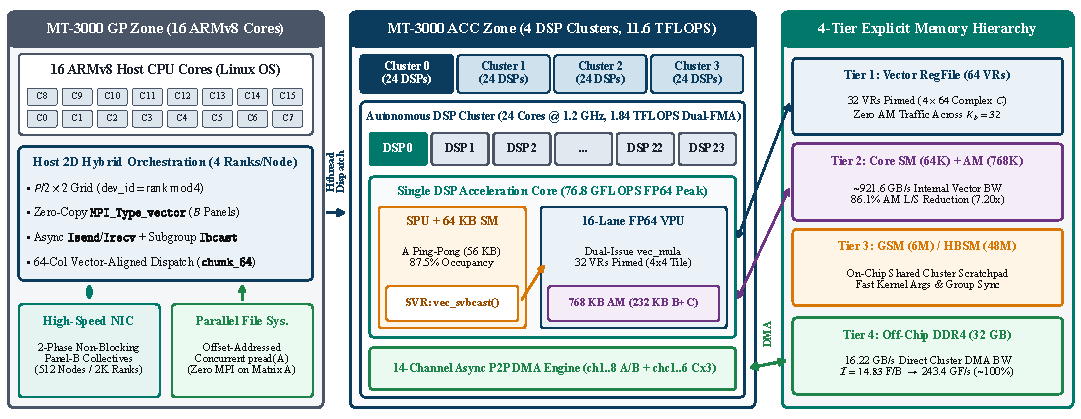
\includegraphics[width=0.64\textwidth]{fig1_arch_overview.pdf}
    \caption{MT-3000 multi-zone heterogeneous node architecture, four-tier software-managed explicit memory hierarchy, and mapping of our end-to-end hierarchical ZGEMM co-design across the 16-core ARMv8 GP Zone and four autonomous 24-core DSP clusters in the ACC Zone.}
    \label{fig:arch}
\end{figure*}

% ============================================================================
\section{Architectural Background and Motivation}
\label{sec:background}
% ============================================================================

\subsection{MT-3000 Multi-Zone Architecture and Memory Hierarchy}
As illustrated in Fig.~\ref{fig:arch} and detailed in Table~\ref{tab:hw_specs}, the MT-3000 processor adopts a heterogeneous multi-zone System-on-Chip (SoC) architecture~\cite{lu2022mt3000}. The \emph{GP Zone} comprises 16 cache-coherent ARMv8 CPU cores running Linux, network stacks, and the MPI runtime. The \emph{ACC Zone} integrates four physically autonomous DSP clusters managed via the lightweight \texttt{Hthread} heterogeneous driver. Because each DSP cluster maintains independent command queues, on-chip shared memories, and DMA controllers without inter-cluster cache coherence, we bind one MPI rank exclusively to each DSP cluster ($\mathrm{dev\_id} = \mathrm{rank} \bmod 4$, four MPI ranks per physical node), eliminating intra-node device contention.

\begin{table}[t]
\centering
\caption{Verified Architectural Parameters of an MT-3000 Compute Node~\cite{lu2022mt3000, qi2025constraint}}
\label{tab:hw_specs}
\renewcommand{\arraystretch}{1.10}
\setlength{\tabcolsep}{3.5pt}
\resizebox{\columnwidth}{!}{%
\begin{tabular}{@{}lll@{}}
\toprule
\textbf{Zone / Tier} & \textbf{Parameter} & \textbf{Verified Specification} \\
\midrule
\multirow{2}{*}{GP Zone} & Host CPU Cores & 16 ARMv8 Cores (Linux OS) \\
 & Rank Mapping & 4 MPI Ranks/Node (4 GP Cores/Rank) \\
\midrule
\multirow{6}{*}{ACC Zone} & DSP Clusters & 4 Autonomous Clusters/Node (1/Rank) \\
 & Cores / Cluster & 24 Bare-Metal VLIW/SIMD Arrays \\
 & Total Node DSPs & 96 DSP Cores (1,536 FP64 VPU Lanes) \\
 & Clock Frequency & 1.2 GHz \\
 & Dual-FMA Peak & 76.8 GF/s per Core; 1.84 TF/s per Cluster \\
 & Chip-Level Peak & 11.6 TFLOPS FP64 \\
\midrule
\multirow{5}{*}{4-Tier Memory} & Vector Regs (VR) & 64 $\times$ 1,024-bit ($16 \times$ FP64) / Core \\
 & Scalar Mem (SM) & 64 KB / Core (SPU + \texttt{vec\_svbcast}) \\
 & Array Mem (AM) & 768 KB / Core ($\sim$921.6 GB/s Vector BW) \\
 & GSM / HBSM & 6 MB GSM/Cluster; 48 MB Shared HBSM \\
 & Off-Chip DDR4 & 32 GB Shared; \textbf{16.22 GB/s} Cluster DMA \\
\bottomrule
\end{tabular}%
}
\end{table}

Each DSP cluster houses 24 bare-metal DSP acceleration cores clocked at $1.2$~GHz. Within every DSP core, a Scalar Processing Unit (SPU) handles control flow, address generation, and scalar loads from its private $64$~KB \emph{Scalar Memory (SM)}, broadcasting scalar operands into a Scalar-Vector Register (SVR) bridge via \texttt{vec\_svbcast}. Coupled to the SPU is a 16-lane FP64 Vector Processing Unit (VPU) equipped with 64 physical 1,024-bit vector registers ($16 \times 64$-bit doubles per register, \texttt{lvector double}) and dual-issue FMA pipelines (\texttt{vec\_mula}), delivering a theoretical vector FMA ceiling of:
\begin{equation}
\mathcal{P}_{\mathrm{core}} = 16 \times 2\,\text{FMA} \times 2\,\text{FLOPs} \times 1.2\,\text{GHz} = 76.8\,\text{GFLOPS},
\label{eq:core_peak}
\end{equation}
or $\mathcal{P}_{\mathrm{cluster}} = 24 \times 76.8 = 1{,}843.2$~GFLOPS per 24-core cluster~\cite{fang2026mtgemm}. The VPU executes wide contiguous vector loads/stores (\texttt{vec\_ld}/\texttt{vec\_st}) exclusively against its private $768$~KB \emph{Array Memory (AM)} at an aggregate internal bandwidth of $\sim\!921.6$~GB/s. Crucially, \textbf{no hardware cache exists between off-chip DDR4 and SM/AM}: all data movement must be explicitly orchestrated by software using point-to-point hardware DMA channels (\texttt{dma\_p2p}), where each cluster's measured direct DDR4 DMA bandwidth is $\mathcal{B}_{\mathrm{DDR}} = 16.22$~GB/s~\cite{qi2025constraint}.

\subsection{Split-Complex Planar Formulation vs.\ Algebraic 3M}
Given complex matrices $A = A_{\mathrm{Re}} + i A_{\mathrm{Im}} \in \mathbb{C}^{M \times K}$, $B = B_{\mathrm{Re}} + i B_{\mathrm{Im}} \in \mathbb{C}^{K \times N}$, and $C = C_{\mathrm{Re}} + i C_{\mathrm{Im}} \in \mathbb{C}^{M \times N}$, ZGEMM computes:
\begin{equation}
\begin{aligned}
C_{\mathrm{Re}} &\leftarrow C_{\mathrm{Re}} + A_{\mathrm{Re}} B_{\mathrm{Re}} - A_{\mathrm{Im}} B_{\mathrm{Im}}, \\
C_{\mathrm{Im}} &\leftarrow C_{\mathrm{Im}} + A_{\mathrm{Re}} B_{\mathrm{Im}} + A_{\mathrm{Im}} B_{\mathrm{Re}}.
\end{aligned}
\label{eq:zgemm_4m}
\end{equation}
Conventional BLAS interfaces (\texttt{cblas\_zgemm}) store complex numbers in interleaved Array-of-Structures (AoS) layout ($[x_0, y_0, x_1, y_1, \dots]$). On 16-lane VPU architectures without zero-overhead de-interleaving load crossbars, AoS forces costly in-register shuffle permutations on every vector load. Conversely, storing real and imaginary components in \emph{split-complex planar} (Structure-of-Arrays, SoA) format aligns 16 consecutive real or imaginary elements directly onto single 128-byte \texttt{vec\_ld} transactions.

While Gauss/Karatsuba 3M methods reduce arithmetic count from $8MNK$ to $6MNK$ FLOPs via $(A_{\mathrm{Re}}+A_{\mathrm{Im}})(B_{\mathrm{Re}}+B_{\mathrm{Im}})$~\cite{vanzee2017complex}, they are ill-suited to scratchpad-constrained DSP supercomputers for two reasons: (i) forming auxiliary matrix sums consumes extra DDR4 memory and DMA bandwidth, which---as shown below---is the true bottleneck rather than FMA throughput; and (ii) subtracting large intermediate products amplifies floating-point rounding error proportionally to $\max(\|A\|\|B\|/\|C\|)$~\cite{higham2002accuracy}. We therefore execute exact 4M accumulation in~\eqref{eq:zgemm_4m} via native dual-issue fused \texttt{vec\_mula} instructions, preserving strict IEEE-754 FP64 accuracy without workspace allocation.

\subsection{Machine Balance Diagnosis: The Scratchpad Memory Wall}
Dividing the 24-core cluster vector peak $\mathcal{P}_{\mathrm{cluster}} = 1{,}843.2$~GFLOPS by its off-chip DDR4 DMA bandwidth $\mathcal{B}_{\mathrm{DDR}} = 16.22$~GB/s exposes a formidable \emph{machine balance ridge point}~\cite{williams2009roofline}:
\begin{equation}
\mathcal{I}_{\mathrm{ridge}} = \frac{\mathcal{P}_{\mathrm{cluster}}}{\mathcal{B}_{\mathrm{DDR}}} = \frac{1{,}843.2\,\text{GFLOPS}}{16.22\,\text{GB/s}} = 113.64\,\text{FLOPs/B}.
\label{eq:ridge}
\end{equation}
However, for a complex tile $(M_b, K_b, N_b)$ buffered inside a core's $64$~KB SM and $768$~KB AM, every $K_b$ step streams $16(M_b K_b + K_b N_b)$ bytes of $A$ and $B$ from DDR4 to perform $8 M_b K_b N_b$ FLOPs, bounding the asymptotic tile arithmetic intensity to $\mathcal{I}_{\max} < \frac{M_b N_b}{2(M_b + N_b)}$. Even if $A$ filled the entire $64$~KB SM ($M_b \approx 64$), $\mathcal{I}_{\max} \le 16$~FLOPs/Byte $\ll 113.64$~FLOPs/Byte. Consequently, \emph{multi-core ZGEMM on MT-3000 is fundamentally DDR4-DMA-bandwidth-bound at the cluster level, yet AM-port- and FMA-latency-bound within each core}. Achieving theoretical hardware limits requires: (1) maximizing tile arithmetic intensity within the $64$~KB SM ceiling while achieving $100\%$ overlap between DDR4 DMA transfers (including $C$ tiles) and VPU execution; and (2) preventing MPI collectives and strong-scaling tile fragmentation from degrading cluster DMA efficiency at scale.

\begin{figure*}[t]
    \centering
    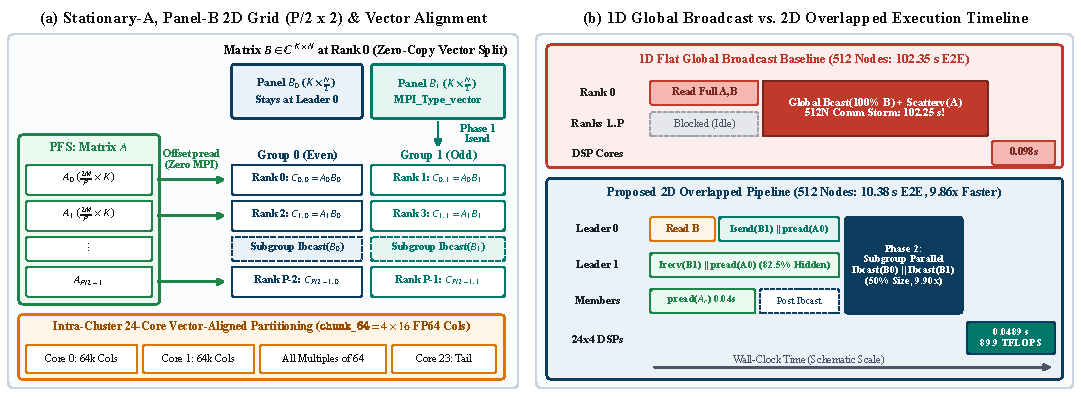
\includegraphics[width=0.64\textwidth]{fig2_2d_comm_timeline.pdf}
    \caption{Proposed Stationary-$A$, Panel-Broadcast-$B$ 2D hybrid orchestration ($P/2 \times 2$): (a) zero-copy strided \texttt{MPI\_Type\_vector} dispatch of $B$ panels, zero-communication offset-addressed parallel \texttt{pread} of $A$ slices, disjoint $C_{r,g}$ ownership without reduction, and 64-column vector-aligned 24-core partitioning; (b) asynchronous execution timeline contrasting the 512-node 1D communication storm against our two-phase overlapped pipeline.}
    \label{fig:comm2d}
\end{figure*}

% ============================================================================
\section{Hierarchical 2D Data Orchestration and Overlapped Collective Pipeline}
\label{sec:host_2d}
% ============================================================================

\subsection{Stationary-$A$, Panel-Broadcast-$B$ 2D Process Grid}
In a conventional 1D row-block baseline (\texttt{gemm\_host\_AS.c}), Rank~0 reads full matrices $A$ and $B$ from storage, scatters $M/P$ rows of $A$ to $P$ ranks via \texttt{MPI\_Scatterv}, and broadcasts $100\%$ of $B$ across \texttt{MPI\_COMM\_WORLD} via \texttt{MPI\_Bcast}. At $P = 2{,}048$ ranks ($512$ nodes), global broadcast contention causes communication latency to explode to $102.25$~s while shrinking per-rank row height to $M_{\mathrm{local}} = 8192 / 2048 = 4$ rows. Conversely, general $\sqrt{P} \times \sqrt{P}$ 2D SUMMA~\cite{vandegeijn1997summa} requires $\sqrt{P}$ iterative broadcast-compute barriers over both $A$ and $B$ panels, repeatedly stalling bare-metal DSP group launches, whereas 2.5D/3D replication~\cite{solomonik2011comm25d} incurs costly post-compute \texttt{MPI\_Allreduce}/\texttt{Reduce\_scatter} over $C$ and exceeds the $32$~GB per-node DDR4 capacity when four ranks share one node.

We design an asymmetric \textbf{Stationary-$A$, Panel-Broadcast-$B$ 2D hybrid topology} organized as a $(P/G) \times G$ logical grid (Fig.~\ref{fig:comm2d}(a) and Algorithm~\ref{alg:host_2d}). Using cyclic subgroup assignment via \texttt{MPI\_Comm\_split}, each global rank $p \in [0, P-1]$ maps to column-panel subgroup $g = p \bmod G$, intra-group row index $r = \lfloor p / G \rfloor \in [0, P_g - 1]$ (where $P_g = P/G$), and physical node DSP cluster $d = p \bmod 4$. Matrix $B \in \mathbb{C}^{K \times N}$ is partitioned column-wise into $G$ disjoint vertical panels $B_g \in \mathbb{C}^{K \times N_g}$ with $N_g = \lfloor N/G \rfloor + \mathbb{I}(g < N \bmod G)$, while matrix $A \in \mathbb{C}^{M \times K}$ is partitioned row-wise into $P_g$ horizontal slices $A_r \in \mathbb{C}^{M_r \times K}$. Because subgroup leader ranks ($r = 0$) bear extra inter-leader dispatch overhead for $B_g$, we employ an asymmetric load-balanced row rule (\texttt{gemm\_host\_AB\_opt6.c}) with remainder $R_M = (M - M_0) \bmod (P_g - 1)$ that shields leaders from remainder rows:
\begin{equation}
M_r = \begin{cases}
\lfloor M / P_g \rfloor, & r = 0, \\[3pt]
\left\lfloor \dfrac{M - M_0}{P_g - 1} \right\rfloor + \mathbb{I}(r \le R_M), & 1 \le r < P_g.
\end{cases}
\label{eq:row_alloc}
\end{equation}
Process $(r, g)$ exclusively computes the disjoint output submatrix $C_{r,g} \leftarrow C_{r,g} + A_r B_g \in \mathbb{C}^{M_r \times N_g}$ directly inside DSP-mapped memory (\texttt{hthread\_malloc}), requiring \textbf{zero network communication of $A$ and zero post-compute reduction of $C$}.

\begin{table*}[t]
\centering
\caption{Asymptotic Per-Rank Complexity Comparison Across Distributed GEMM Topologies ($P$ Ranks, Square Scale $M=N=K$, $G$ Panels)}
\label{tab:complexity}
\renewcommand{\arraystretch}{1.14}
\setlength{\tabcolsep}{5.0pt}
\resizebox{\textwidth}{!}{%
\begin{tabular}{@{}lccccc@{}}
\toprule
\textbf{Distributed Scheme} & \textbf{Network Volume ($A + B + C$)} & \textbf{Collective Sync Stages} & \textbf{File I/O Critical Path} & \textbf{Local Rows $M_{\mathrm{local}}$} & \textbf{DDR-Streaming Floor $T_{\mathrm{stream}}$} \\
\midrule
1D Flat Broadcast (\texttt{AS}) & $16\frac{N^2}{P} + 16 N^2 \log_2 P + 0$ & $2$ Global ($\log_2 P$) & $\mathcal{O}(N^2)$ Serialized at Root & $N / P$ & $\ge 16 N^2 / \mathcal{B}_{\mathrm{DDR}}$ \\
2D SUMMA ($\sqrt{P} \times \sqrt{P}$)~\cite{vandegeijn1997summa} & $\frac{32 N^2}{\sqrt{P}} \log_2 \sqrt{P}$ & $\frac{2N}{K_{\mathrm{panel}}} \log_2 \sqrt{P}$ Iterative & $\mathcal{O}(N^2)$ or MPI-IO & $N / \sqrt{P}$ & Iterative Launch Overhead \\
2.5D Replication ($c$ copies)~\cite{solomonik2011comm25d} & $\frac{32 N^2}{\sqrt{P c}}\log_2\!\sqrt{\frac{P}{c}} + \frac{16 N^2 \log_2 c}{P/c}$ & $\sqrt{\frac{P}{c^3}}$ Bcast + Allreduce & $\mathcal{O}(N^2)$ + $c\times$ Mem Footprint & $N \sqrt{c / P}$ & Extra $C$-Reduction Traffic \\
\textbf{Proposed Stationary-$A$ ($P/G \times G$)} & $\mathbf{0 + \frac{16 N^2}{G} \log_2\!\left(\frac{P}{G}\right) + 0}$ & \textbf{1 Async Subgroup ($\log_2 \frac{P}{G}$)} & \textbf{$\mathcal{O}\!\left(\frac{G N^2}{P}\right)$ Overlapped \texttt{pread}} & $\mathbf{G N / P}$ & $\mathbf{\ge \frac{16 N^2}{G \cdot \mathcal{B}_{\mathrm{DDR}}}}$ (\textbf{$G\times$ Lower Floor}) \\
\bottomrule
\end{tabular}%
}
\end{table*}

\subsection{Zero-Copy Strided Vector Dispatch and Two-Phase Collectives}
Because $B$ is stored in row-major order, column panels $B_g$ ($g \ge 1$) consist of $K$ non-contiguous segments of width $N_g$ separated by stride $N$. Packing $B_g$ into intermediate contiguous host buffers at Rank~0 would consume gigabytes of scarce node RAM and pollute memory bandwidth. Instead, Rank~0 constructs and commits a zero-copy derived strided datatype (\texttt{operator.c}):
\begin{equation}
\mathcal{D}_{B_g} \triangleq \texttt{MPI\_Type\_vector}(K,\; N_g,\; N,\; \texttt{MPI\_DOUBLE}),
\label{eq:mpi_vector}
\end{equation}
and dispatches $B_g$ directly from the in-place column offset $\&B[0, j_{\mathrm{start}}(g)]$ to each subgroup leader ($r=0, g \ge 1$) via non-blocking \texttt{MPI\_Isend}, which the receiving leader unpacks on-the-fly into a contiguous DSP-mapped buffer of layout $(K, N_g)$ via \texttt{MPI\_Irecv} (Phase~1). Immediately upon Phase-1 completion, all $G$ subgroup leaders concurrently execute non-blocking \texttt{MPI\_Ibcast} of their half-width contiguous panels $B_g$ across isolated subgroup communicators $\mathcal{C}_g$ of size $P/G$ (Phase~2).

Under the Rabenseifner binomial/scatter-allgather collective cost model~\cite{thakur2005mpich} with startup latency $\alpha$, per-byte transfer time $\beta$, and network contention penalty $\gamma(P)$ that grows superlinearly when switch buffers saturate at scale, 1D global broadcast versus our 2D subgroup broadcast satisfies:
\begin{equation}
\begin{aligned}
T_{\mathrm{comm}}^{\mathrm{1D}}(P) &= \alpha \log_2 P + 32 K N \left(\beta + \gamma(P)\right), \\
T_{\mathrm{comm}}^{\mathrm{2D}}(P, G) &= T_{\mathrm{p2p}}(G) + \alpha \log_2\!\left(\frac{P}{G}\right) \\
&\quad + \frac{32 K N}{G}\!\left(\beta + \gamma\!\left(\frac{P}{G}\right)\right).
\end{aligned}
\label{eq:comm_cost}
\end{equation}
Setting $G=2$ simultaneously halves the broadcast payload ($1.074$~GB $\to 0.537$~GB at $N=8192$), halves the collective fan-out ($2{,}048 \to 1{,}024$ ranks per isolated tree), and eliminates cross-tree switch contention, collapsing 512-node communication time by $9.90\times$ (Section~\ref{sec:eval_scaling}). Table~\ref{tab:complexity} summarizes the asymptotic advantages over 1D, SUMMA, and 2.5D schemes.

\begin{algorithm}[t]
\caption{Host-Side 2D Hybrid Orchestration \& Overlapped Pipeline}
\label{alg:host_2d}
\footnotesize
\begin{algorithmic}[1]
\REQUIRE Dimensions $(M, K, N)$, total ranks $P$, panel groups $G=2$, rank $p$.
\ENSURE Distributed disjoint submatrices $C_{r,g} = C_{r,g} + A_r B_g$ in DSP memory.
\STATE Bind rank to autonomous DSP cluster: $d \leftarrow p \bmod 4$; \texttt{hthread\_dev\_open}$(d)$.
\STATE Split communicator: $g \leftarrow p \bmod G$, $r \leftarrow \lfloor p / G \rfloor$, $\mathcal{C}_g \leftarrow$ \texttt{MPI\_Comm\_split}$(g, r)$.
\STATE Compute local dimensions $(M_r, N_g)$ and row offset $i_0(r)$ via~\eqref{eq:row_alloc}.
\STATE Allocate DSP-pinned buffers $A_r \in \mathbb{C}^{M_r \times K}, B_g \in \mathbb{C}^{K \times N_g}, C_{r,g} \in \mathbb{C}^{M_r \times N_g}$.
\IF{$p = 0$}
    \STATE Load $B_{\mathrm{Re}}, B_{\mathrm{Im}}$; commit strided $\mathcal{D}_{B_{g'}}$ via~\eqref{eq:mpi_vector}; post \texttt{MPI\_Isend} to leaders $g' \in [1, G-1]$; extract local $B_0$. \COMMENT{Phase-1 async send}
\ELSIF{$r = 0$ \AND $g > 0$}
    \STATE Post non-blocking \texttt{MPI\_Irecv} for $B_{\mathrm{Re},g}, B_{\mathrm{Im},g}$ from Rank~0.
\ENDIF
\STATE \textbf{Concurrently} execute offset-addressed \texttt{pread64} of $A_{\mathrm{Re},r}, A_{\mathrm{Im},r}$ at byte offset $8 \cdot i_0(r) \cdot K$ into \texttt{HT\_MEM\_RO} buffer $A_r$. \COMMENT{Overlaps Phase-1 NIC}
\IF{$r = 0$}
    \STATE \texttt{MPI\_Waitall} on Phase-1 handles; post \texttt{MPI\_Ibcast}$(B_g, \mathcal{C}_g)$.
\ELSE
    \STATE Post \texttt{MPI\_Ibcast}$(B_g, \mathcal{C}_g)$ immediately after \texttt{pread64}. \COMMENT{Phase-2 tree}
\ENDIF
\STATE Compute 64-col vector-aligned 24-core partition $\{N_{\mathrm{thread}}(t)\}_{t=0}^{23}$ via~\eqref{eq:chunk64}.
\STATE \texttt{MPI\_Waitall} on Phase-2 \texttt{Ibcast}; launch 24-core DSP group (Algorithm~\ref{alg:device_kernel}).
\end{algorithmic}
\end{algorithm}

\subsection{Concurrent Sliced \texttt{pread} and Communication-I/O Overlap}
Rather than reading $A$ at Rank~0 and scattering over MPI, every rank $(r, g)$ computes its exact byte offset $\Delta_r = 8 \cdot i_0(r) \cdot K$ and invokes POSIX \texttt{pread64} (\texttt{read\_data.c}) to stream its $M_r \times K$ slice directly from the parallel file system into Hthread DMA-mapped read-only memory (\texttt{HT\_MEM\_RO}). As shown in Fig.~\ref{fig:comm2d}(b) and Lines~6--15 of Algorithm~\ref{alg:host_2d}, subgroup leaders issue \texttt{pread64} \emph{after} posting Phase-1 \texttt{MPI\_Isend}/\texttt{MPI\_Irecv} requests and \emph{before} \texttt{MPI\_Waitall}, overlapping host file-system DMA with RDMA network progress. Non-leader members ($r \ge 1$) read $G/P$ of matrix $A$ in parallel without root serialization and immediately post non-blocking \texttt{MPI\_Ibcast} to join the subgroup tree.

\subsection{64-Column Vector-Aligned Partitioning and Optimality of $G=2$}
Within each cluster, $N_g$ columns of $B_g$ and $C_{r,g}$ are distributed across $T = 24$ DSP cores. Because our micro-kernel (Section~\ref{sec:device}) processes tiles of width $N_b = 64 = 4 \times 16$ columns, any core assigned a non-multiple of $64$ columns suffers misaligned tail blocks requiring scalar SPU zero-padding loops (\texttt{N\_cur != N\_block}). We enforce a strict \textbf{64-column vector-aligned partitioning} (\texttt{chunk\_64 = 64}): letting $Q = \lfloor N_g / 64 \rfloor$, $q = \lfloor Q / 24 \rfloor$, and $u = Q \bmod 24$, core $t \in [0, 23]$ receives:
\begin{equation}
N_{\mathrm{thread}}(t) = \begin{cases}
64(q + 1), & 0 \le t < u, \\
64 q, & u \le t < 23, \\
64 q + (N_g \bmod 64), & t = 23.
\end{cases}
\label{eq:chunk64}
\end{equation}
When $64 \mid N_g$, \emph{all 24 DSP cores} execute exclusively on full 64-column vector tiles without scalar tails.

Equation~\eqref{eq:chunk64} also yields a closed-form proof for why \textbf{$G = 2$ is the unique optimal panel group count} for $N = 8192$ on 24-core MT-3000 clusters:
\begin{itemize}\setlength{\itemsep}{1pt}\setlength{\parskip}{0pt}
    \item \emph{Full 24-Core Active Occupancy Constraint:} Keeping all 24 cores active on $\ge 1$ full 64-column block requires $N_g = N/G \ge 24 \times 64 = 1{,}536 \implies G \le 5.33$. Any $G \ge 8$ ($N_g \le 1{,}024 = 16 \times 64$) leaves at least $8$ of $24$ DSP cores ($33.3\%$) completely idle.
    \item \emph{Three-Stage $C$-Buffer Pipeline Constraint:} Sustaining cyclic triple-buffer rotation of $C$ (Section~\ref{sec:device}) requires $N_{\mathrm{thread}}(t) \ge 3 N_b = 192$ columns ($Q \ge 72$) across the majority of cores. For $G = 4$, $N_g = 2{,}048$ ($Q = 32$), forcing $16$ of $24$ cores down to $N_{\mathrm{thread}} = 64$ (a single tile), disabling outer $C$-DMA overlap.
    \item \emph{Optimal Balance at $G = 2$:} $N_g = 4{,}096$ ($Q = 64$, $64 \mid N_g$) assigns $192$ columns ($3$ tiles) to $16$ cores and $128$ columns ($2$ tiles) to $8$ cores with zero tail padding, while doubling $M_{\mathrm{local}} = 2M/P$ over $G=1$ and halving both broadcast volume and the DDR-streaming floor.
\end{itemize}

\begin{figure*}[t]
    \centering
    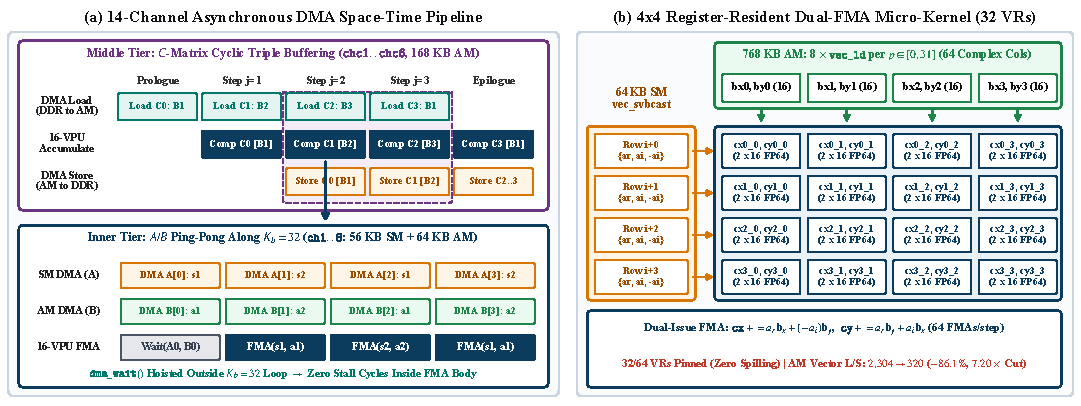
\includegraphics[width=0.64\textwidth]{fig3_tri_pipeline_microkernel.pdf}
    \caption{Intra-chip scratchpad and register co-design: (a) 14-channel asynchronous P2P DMA space-time pipeline nesting inner-tier $A/B$ ping-pong double buffering (\texttt{ch1..ch8}) inside middle-tier $C$-matrix cyclic triple buffering (\texttt{chc1..chc6}); (b) $4 \times 4$ vector-register-resident outer-product dual-FMA micro-kernel pinning 32 physical vector accumulators to eliminate $86.1\%$ of Array Memory vector load/store traffic.}
    \label{fig:microkernel}
\end{figure*}

% ============================================================================
\section{Tri-Buffered Scratchpad Pipeline and $4 \times 4$ Register-Resident Micro-Kernel}
\label{sec:device}
% ============================================================================

\subsection{14-Channel Asynchronous DMA Tri-Buffered State Machine}
On bare-metal DSP cores lacking hardware caches, conventional $A/B$ ping-pong double buffering leaves the DDR4 read and write-back latencies of each $M_b \times N_b$ complex $C$ tile ($112$~KB round-trip) unhidden between $K$-reduction loops. Worse, reusing only two $C$ buffers creates a Read-After-Write / Write-After-Read hazard: at outer step $j$, the DMA engine must concurrently \emph{write back} completed $C^{(j-1)}$ to DDR4, \emph{accumulate} active $C^{(j)}$ on the VPU, and \emph{prefetch} upcoming $C^{(j+1)}$ from DDR4.

We resolve this hazard via a \textbf{14-channel two-tier software-pipelined DMA state machine} (\texttt{matrix\_mul\_pipeline\_opt} in \texttt{kernel\_pipeline.c}; Fig.~\ref{fig:microkernel}(a) and Algorithm~\ref{alg:device_kernel}):
\begin{enumerate}\setlength{\itemsep}{0.5pt}\setlength{\parskip}{0pt}
    \item \textbf{Middle-Tier $C$-Matrix Cyclic Triple Buffering (6 Channels, \texttt{chc1..chc6}):} Three split-complex buffer pairs $\{(\texttt{Cx\_a}_s, \texttt{Cy\_a}_s)\}_{s=1}^{3}$ reside in AM ($168$~KB total). Across column-tile steps $j = 0, N_b, 2N_b, \dots$, cyclic rotation maps buffer $(j/N_b) \bmod 3$ to prefetch $C^{(j)}$ via strided P2P DMA (\texttt{dma\_p2p}), buffer $(j/N_b - 1) \bmod 3$ to VPU $K$-accumulation, and buffer $(j/N_b - 2) \bmod 3$ to asynchronous DDR4 write-back of $C^{(j-2N_b)}$, hiding $100\%$ of bidirectional $C$ DDR4 traffic behind the $\lceil K / K_b \rceil$ inner FMA stages.
    \item \textbf{Inner-Tier $A/B$ Ping-Pong Double Buffering (8 Channels, \texttt{ch1..ch8}):} Along $K$, two complex $A$ buffer pairs $\{(\texttt{Ax\_s}_1, \texttt{Ay\_s}_1), (\texttt{Ax\_s}_2, \texttt{Ay\_s}_2)\}$ reside in $64$~KB SM (\texttt{ch1..ch4}, $56$~KB), while two complex $B$ buffer pairs $\{(\texttt{Bx\_a}_1, \texttt{By\_a}_1), (\texttt{Bx\_a}_2, \texttt{By\_a}_2)\}$ reside in $768$~KB AM (\texttt{ch5..ch8}, $64$~KB). Before entering the $4 \times 4$ micro-kernel on buffer pair $b \in \{1, 2\}$, the SPU posts non-blocking \texttt{dma\_p2p} prefetches for step $k + K_b$ into alternate pair $3 - b$, hoisting all \texttt{dma\_wait} barriers strictly \emph{outside} the inner $K_b=32$ FMA loop.
\end{enumerate}

\begin{algorithm}[t]
\caption{Device-Side 14-Channel Tri-Buffered DSP Kernel}
\label{alg:device_kernel}
\footnotesize
\begin{algorithmic}[1]
\REQUIRE Submatrices $A \in \mathbb{C}^{M_r \times K}, B \in \mathbb{C}^{K \times N_g}, C \in \mathbb{C}^{M_r \times N_g}$; core ID $t \in [0, 23]$; tile $(M_b, K_b, N_b) = (56, 32, 64)$.
\ENSURE Updated core slice $C[:, j_0(t) : j_0(t)+N_{\mathrm{thread}}(t)]$.
\STATE Allocate SM ping-pong $\{Ax_{1,2}, Ay_{1,2}\}$ ($56$~KB) and AM buffers $\{Bx_{1,2}, By_{1,2}\}$ ($64$~KB) + cyclic triple buffers $\{Cx_{1..3}, Cy_{1..3}\}$ ($168$~KB).
\FOR{$i = 0$ \TO $M_r - 1$ \textbf{step} $M_b$}
    \STATE \textbf{Prologue ($j=0$):} Async \texttt{dma\_p2p} load $C[i, j_0]$ into $(Cx_1, Cy_1)$.
    \FOR{$j = N_b$ \TO $N_{\mathrm{thread}}(t) - 1$ \textbf{step} $N_b$}
        \STATE Rotate $(s_{\mathrm{store}}, s_{\mathrm{comp}}, s_{\mathrm{load}})$ mod $3$; post async \texttt{dma\_p2p} prefetch of $C[i, j_0+j]$ into $(Cx_{s_{\mathrm{load}}}, Cy_{s_{\mathrm{load}}})$.
        \STATE Post async \texttt{dma\_p2p} for $A[i, 0] \to (Ax_1, Ay_1)$ and $B[0, j_0+j-N_b] \to (Bx_1, By_1)$; \texttt{dma\_wait} on $C_{s_{\mathrm{comp}}}$ and prior $C_{s_{\mathrm{store}}}$.
        \FOR{$k_{\mathrm{idx}} = 0$ \TO $\lceil K / K_b \rceil - 1$}
            \STATE $b \leftarrow (k_{\mathrm{idx}} \bmod 2) + 1$; $\bar{b} \leftarrow 3 - b$.
            \IF{$k_{\mathrm{idx}} + 1 < \lceil K / K_b \rceil$}
                \STATE Post async \texttt{dma\_p2p} prefetch $A_{k+K_b} \to (Ax_{\bar{b}}, Ay_{\bar{b}})$ (\texttt{ch1..4}) and $B_{k+K_b} \to (Bx_{\bar{b}}, By_{\bar{b}})$ (\texttt{ch5..8}).
            \ENDIF
            \STATE \texttt{dma\_wait} on active $(Ax_b, Ay_b, Bx_b, By_b)$.
            \FOR{$r_0 = 0$ \TO $M_{\mathrm{cur}} - 1$ \textbf{step} $4$}
                \STATE Load 32 VRs $\{\mathbf{cx}_{u,v}, \mathbf{cy}_{u,v}\}_{u,v=0}^{3}$ from $(Cx_{s_{\mathrm{comp}}}, Cy_{s_{\mathrm{comp}}})$.
                \FOR{$p = 0$ \TO $K_{\mathrm{cur}} - 1$}
                    \STATE Load $8$ vectors $\{\mathbf{bx}_v, \mathbf{by}_v\}_{v=0}^{3}$ via \texttt{vec\_ld} from $(Bx_b, By_b)$.
                    \FOR{$u = 0$ \TO $3$}
                        \STATE Broadcast $\{a_r, a_i, -a_i\}$ via \texttt{vec\_svbcast}; execute $8$ dual-issue \texttt{vec\_mula} updates~\eqref{eq:vec_mula}.
                    \ENDFOR
                \ENDFOR
                \STATE Store 32 VRs $\{\mathbf{cx}_{u,v}, \mathbf{cy}_{u,v}\}$ to $(Cx_{s_{\mathrm{comp}}}, Cy_{s_{\mathrm{comp}}})$.
            \ENDFOR
        \ENDFOR
        \STATE Post async \texttt{dma\_p2p} store $(Cx_{s_{\mathrm{comp}}}, Cy_{s_{\mathrm{comp}}}) \to C[i, j_0+j-N_b]$.
    \ENDFOR
    \STATE \textbf{Epilogue:} Accumulate final $j$-tile and \texttt{dma\_wait} final $C$ write-backs.
\ENDFOR
\end{algorithmic}
\end{algorithm}

\subsection{$4 \times 4$ Vector-Register-Resident Dual-FMA Micro-Kernel}
Even after operands reside in SM and AM, naive loop ordering ($p \to i \to v$) loads and stores $C_{\mathrm{Re}}$ and $C_{\mathrm{Im}}$ vectors from AM at every $p \in [0, K_b - 1]$ step. For a $4 \times 64$ complex sub-tile over $K_b = 32$ steps, naive inner-loop accumulation issues $32 \times (8~\text{B-loads} + 4 \times 8~\text{C-loads} + 4 \times 8~\text{C-stores}) = 2{,}304$ AM vector memory instructions for $2{,}048$ vector FMAs ($0.89$ FMAs per AM access), causing severe AM port contention.

To break this bottleneck, we design a \textbf{$4 \times 4$ outer-product register-resident micro-kernel} (\texttt{COMPUTE\_K\_BLOCK\_OPT\_C}, Fig.~\ref{fig:microkernel}(b)):
\begin{itemize}\setlength{\itemsep}{1pt}\setlength{\parskip}{0pt}
    \item \textbf{Exact 32-VR Accumulator Pinning (Zero Spilling):} We unroll $4$ rows along $M_b$ and $4$ vector segments ($4 \times 16 = 64$ complex columns) along $N_b$, allocating $4 \times 4 \times 2 = \mathbf{32}$ physical vector registers ($\mathbf{cx}_{u,v}, \mathbf{cy}_{u,v}$ for $u,v \in \{0,1,2,3\}$) to hold the $4 \times 64$ complex $C$ sub-tile. Together with $8$ streaming $B$ vector registers ($\mathbf{bx}_{0..3}, \mathbf{by}_{0..3}$) and $3$ scalar-broadcast $A$ registers ($\tilde{\mathbf{a}}_r, \tilde{\mathbf{a}}_i, -\tilde{\mathbf{a}}_i$), total live register occupancy is $43$ out of $64$ physical VRs ($67.2\%$), guaranteeing \textbf{zero compiler register spilling} to AM.
    \item \textbf{Hoisted SPU Negation for Pure Dual-Issue \texttt{vec\_mula}:} Because $-A_{\mathrm{Im}} B_{\mathrm{Im}}$ in~\eqref{eq:zgemm_4m} involves subtraction, using separate vector multiply and subtract instructions would forfeit dual-issue FMA throughput. Instead, for each row $i+u$, the SPU computes $-a_i$ in scalar arithmetic at zero VPU cost and broadcasts the triplet $\{a_r, a_i, -a_i\}$ across all 16 lanes via \texttt{vec\_svbcast}, enabling all $32$ real and $32$ imaginary updates per $p$-step to execute exclusively as fused dual-issue \texttt{vec\_mula} instructions:
    \begin{equation}
    \begin{aligned}
    \mathbf{cx}_{u,v} &\leftarrow \texttt{vec\_mula}(\tilde{\mathbf{a}}_{r,u},\, \mathbf{bx}_v,\, \mathbf{cx}_{u,v}), \\
    \mathbf{cx}_{u,v} &\leftarrow \texttt{vec\_mula}(-\tilde{\mathbf{a}}_{i,u},\, \mathbf{by}_v,\, \mathbf{cx}_{u,v}), \\
    \mathbf{cy}_{u,v} &\leftarrow \texttt{vec\_mula}(\tilde{\mathbf{a}}_{r,u},\, \mathbf{by}_v,\, \mathbf{cy}_{u,v}), \\
    \mathbf{cy}_{u,v} &\leftarrow \texttt{vec\_mula}(\tilde{\mathbf{a}}_{i,u},\, \mathbf{bx}_v,\, \mathbf{cy}_{u,v}).
    \end{aligned}
    \label{eq:vec_mula}
    \end{equation}
    \item \textbf{$86.1\%$ AM Vector Traffic Elimination:} Across $K_b = 32$ steps, $\mathbf{cx}_{u,v}$ and $\mathbf{cy}_{u,v}$ are loaded once before $p=0$ ($32$ \texttt{vec\_ld}) and stored once after $p=31$ ($32$ \texttt{vec\_st}), while streaming $32 \times 8 = 256$ $B$-vectors. Total AM vector memory instructions drop from $2{,}304$ to $32 + 256 + 32 = \mathbf{320}$---an \textbf{$86.1\%$ reduction ($7.20\times$ fewer AM accesses)}---raising inner-loop intensity to $64 / 8 = \mathbf{8.0}$ vector FMAs per vector load.
\end{itemize}

\subsection{Scratchpad Capacity Proof and Roofline Optimality of $(56, 32, 64)$}
Selecting $(M_b, K_b, N_b)$ is governed by coupled hardware constraints over SM ($64$~KB) and AM ($768$~KB):
\begin{subequations}
\begin{align}
\mathcal{S}_{\mathrm{SM}} &= 2_{\mathrm{buf}} \times 2_{\mathbb{C}} \times M_b K_b \times 8~\text{B} \le 64~\text{KB} - \Delta_{\mathrm{stack}}, \label{eq:sm_cap} \\
\mathcal{S}_{\mathrm{AM}} &= \left(4 K_b N_b + 6 M_b N_b\right) \times 8~\text{B} \le 768~\text{KB}, \label{eq:am_cap} \\
M_b &\equiv 0 \pmod 4, \quad N_b \equiv 0 \pmod{64}, \label{eq:div_cap}
\end{align}
\end{subequations}
where $\Delta_{\mathrm{stack}} \approx 8$~KB reserves SM space for SPU stack frames, DMA descriptors, and kernel control structures, and~\eqref{eq:div_cap} eliminates register-tile remainder branches. Fixing $N_b = 64$ ($4$ vector widths) and $K_b = 32$ (amortizing $C$ register load/store overhead to $64/320 = 20\%$ of AM traffic while keeping SM footprint compact),~\eqref{eq:sm_cap} restricts $M_b \le \frac{56 \times 1024}{32 \times 32} = 56$. Choosing $(M_b, K_b, N_b) = \mathbf{(56, 32, 64)}$ yields:
\begin{itemize}\setlength{\itemsep}{1pt}\setlength{\parskip}{0pt}
    \item $\mathcal{S}_{\mathrm{SM}} = 4 \times 56 \times 32 \times 8 = \mathbf{56.0~\text{KB}}$ (\textbf{$87.5\%$ of $64$~KB SM}, exact $8.0$~KB control headroom, and $56 = 14 \times 4$ exact $4$-row micro-tiles with zero row remainder);
    \item $\mathcal{S}_{\mathrm{AM}} = (4 \times 32 \times 64 + 6 \times 56 \times 64) \times 8 = 64.0 + 168.0 = \mathbf{232.0~\text{KB}}$ ($30.2\%$ of $768$~KB AM).
\end{itemize}

For reduction length $K$, processing one $(M_b, N_b)$ output tile executes $8 M_b K N_b$ FLOPs while transferring $16 K (M_b + N_b) + 32 M_b N_b$ bytes across the DDR4 DMA bus, yielding operational arithmetic intensity (at $K=8192$):
\begin{equation}
\mathcal{I}_{\mathrm{DMA}} = \frac{8 M_b K N_b}{16 K (M_b + N_b) + 32 M_b N_b} = \mathbf{14.83\,\text{FLOPs/B}},
\label{eq:ai_dma}
\end{equation}
(asymptotic limit $14.93$~FLOPs/Byte). Multiplying by the measured cluster DDR4 DMA bandwidth $\mathcal{B}_{\mathrm{DDR}} = 16.22$~GB/s~\cite{qi2025constraint} defines the \textbf{theoretical 24-core cluster Roofline ceiling}:
\begin{equation}
\mathcal{P}_{\mathrm{roof}}^{\mathrm{cluster}} = \mathcal{B}_{\mathrm{DDR}} \times \mathcal{I}_{\mathrm{DMA}} = 16.22 \times 14.83 = \mathbf{240.5~\text{GFLOPS}}.
\label{eq:cluster_roofline}
\end{equation}

\subsection{Strong-Scaling Off-Chip DDR-Streaming Floor Theorem}
Equation~\eqref{eq:ai_dma} assumes $M_{\mathrm{local}} \ge M_b = 56$. During strong scaling of fixed problem size $(M, K, N)$ across $P$ ranks with $G$ panel subgroups, each rank holds $M_{\mathrm{local}}(P, G) = G M / P$ rows. Once $P > G M / M_b$ ($P > 146$ for 1D $G=1$; $P > 292$ for 2D $G=2$ at $M=8192$), the effective tile height clamps to $M_{\mathrm{eff}} = M_{\mathrm{local}} < 56$, causing operational arithmetic intensity to collapse to:
\begin{equation}
\mathcal{I}_{\mathrm{eff}}(P, G) \approx \frac{M_{\mathrm{local}} N_b}{2\left(M_{\mathrm{local}} + N_b\right)}.
\label{eq:ai_collapse}
\end{equation}
At 512 nodes ($P = 2{,}048$), 1D partitioning ($G=1, M_{\mathrm{local}}=4$) degrades to $\mathcal{I}_{\mathrm{eff}} = \mathbf{1.88~\text{FLOPs/Byte}}$, whereas our 2D hybrid topology ($G=2, M_{\mathrm{local}}=8$) sustains $\mathcal{I}_{\mathrm{eff}} = \mathbf{3.56~\text{FLOPs/Byte}}$ ($1.89\times$ higher). Equivalently, because every cluster must stream its assigned $B_g \in \mathbb{C}^{K \times (N/G)}$ panel ($16 K N / G$ bytes) from DDR4 at least once, kernel wall time obeys the fundamental \textbf{DDR-streaming lower bound} $T_{\mathrm{stream}}(G)$:
\begin{equation}
T_{\mathrm{kernel}}(P, G) \ge \frac{16 K (N / G) + 16 M_{\mathrm{local}}(K + 2 N / G)}{\mathcal{B}_{\mathrm{DDR}}}.
\label{eq:ddr_floor}
\end{equation}
As $P \to \infty$ ($M_{\mathrm{local}} \ll N/G$), $T_{\mathrm{stream}}(1) / T_{\mathrm{stream}}(2) \to \mathbf{2.00\times}$ ($1.074$~GB/$16.22$~GB/s $\approx 0.066$~s pure-$B$ floor plus pipeline prologue/epilogue), predicting the $2.01\times$ kernel speedup ($0.0982$~s $\to 0.0489$~s) measured at 512 nodes for $N=8192$. Moreover, doubling problem dimension to $N=16384$ at 512 nodes ($P=2{,}048, G=2$) raises $M_{\mathrm{local}}$ from $8$ to $16$ rows and $\mathcal{I}_{\mathrm{eff}}$ in~\eqref{eq:ai_collapse} from $3.56$ to $\mathbf{6.40~\text{FLOPs/Byte}}$, yielding an analytical 512-node Roofline prediction of $2{,}048 \times 16.22 \times 6.39 = \mathbf{212.3~\text{TFLOPS}}$ that closely predicts our measured $218.79$~TFLOPS ($0.1608$~s).

% ============================================================================
\section{Experimental Evaluation}
\label{sec:eval}
% ============================================================================

\begin{table*}[t]
\centering
\caption{Intra-Node Performance (GFLOPS), Speedup, and FP64 Numerical Accuracy ($\ell_\infty$ Error) vs.\ Multi-Threaded ARMv8 OpenBLAS}
\label{tab:intra_node}
\renewcommand{\arraystretch}{1.08}
\setlength{\tabcolsep}{4.0pt}
\resizebox{\textwidth}{!}{%
\begin{tabular}{@{}rcccccccccccc@{}}
\toprule
 & \multicolumn{4}{c}{\textbf{Single-Core Compute Density (1 Core)}} & \multicolumn{6}{c}{\textbf{Cluster-Level Throughput (1 DSP Cluster [24C] vs.\ Multi-Core CPU)}} & \multicolumn{2}{c}{\textbf{FP64 Max Error ($\ell_\infty$)}} \\
\cmidrule(lr){2-5} \cmidrule(lr){6-11} \cmidrule(l){12-13}
\textbf{Scale $N$} & \textbf{DSP 1C} & \textbf{CPU 1C} & \textbf{CPU 1C} & \textbf{Speedup} & \textbf{DSP 24C} & \textbf{CPU 4C} & \textbf{CPU 16C} & \textbf{CPU 16C} & \textbf{vs.\ 4C} & \textbf{vs.\ 16C} & $\max|\Delta C_{\mathrm{Re}}|$ & $\max|\Delta C_{\mathrm{Im}}|$ \\
($M\!=\!N\!=\!K$) & \textbf{Ours} & \texttt{4xDGEMM} & \texttt{1xZGEMM} & (\texttt{4D} / \texttt{1Z}) & \textbf{(1 Clust.)} & \texttt{4xDGEMM} & \texttt{4xDGEMM} & \texttt{1xZGEMM} & (\textbf{Clust-Eq}) & (\texttt{4D} / \texttt{1Z}) & (Real Part) & (Imag Part) \\
\midrule
$512$ & \textbf{44.16} & 7.22 & 7.10 & $6.12\times$ / $6.22\times$ & \textbf{80.98} & 23.32 & 17.23 & 40.99 & $3.47\times$ & $4.70\times$ / $1.98\times$ & $7.28\times 10^{-12}$ & $1.13\times 10^{-10}$ \\
$1{,}024$ & \textbf{45.77} & 7.07 & 7.69 & $6.48\times$ / $5.95\times$ & \textbf{139.73} & 28.38 & 51.88 & 82.29 & $4.92\times$ & $2.69\times$ / $1.70\times$ & $1.73\times 10^{-11}$ & $3.27\times 10^{-10}$ \\
$2{,}048$ & \textbf{49.19} & 6.80 & 7.63 & $7.24\times$ / $6.45\times$ & \textbf{145.96} & 22.84 & 86.15 & 92.49 & $6.39\times$ & $1.69\times$ / $1.58\times$ & $4.37\times 10^{-11}$ & $9.75\times 10^{-10}$ \\
$4{,}096$ & \textbf{48.39} & 6.78 & 7.74 & $7.13\times$ / $6.25\times$ & \textbf{173.05} & 24.41 & 92.28 & 85.51 & $7.09\times$ & $1.88\times$ / $2.02\times$ & $7.46\times 10^{-11}$ & $2.79\times 10^{-9}$ \\
$8{,}192$ & \textbf{49.16} & 6.76 & 7.60 & $\mathbf{7.28\times}$ / $\mathbf{6.47\times}$ & \textbf{243.44} & 26.08 & 44.56 & 89.65 & $\mathbf{9.33\times}$ & $5.46\times$ / $\mathbf{2.72\times}$ & $1.89\times 10^{-10}$ & $7.57\times 10^{-9}$ \\
$16{,}384^{\dagger}$ & \textbf{49.16} & 7.20 & OOM & $6.83\times$ / --- & \textbf{199.21} & 26.62 & 30.34 & OOM & $7.48\times$ & $\mathbf{6.57\times}$ / --- & $1.05\times 10^{-9}$ & $2.18\times 10^{-8}$ \\
\bottomrule
\end{tabular}%
}
\vspace{1pt}
\par{\raggedright\scriptsize $^{\dagger}$At $N=16384$, allocating $12$~GiB of interleaved AoS buffers alongside planar host and Hthread DMA buffers exceeds $32$~GB node DDR4; single-cluster evaluation executes via $2 \times 2$ host-tiled scheduling without AoS workspace.\par}
\end{table*}

\begin{figure*}[t]
    \centering
    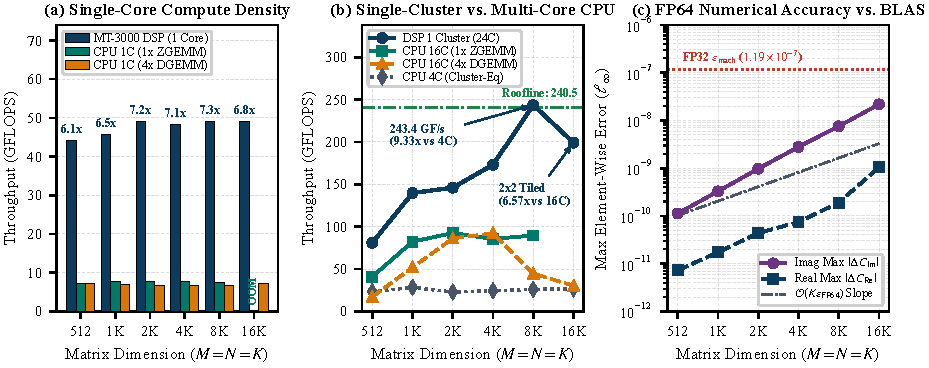
\includegraphics[width=0.64\textwidth]{fig4_intra_node_openblas.pdf}
    \caption{Intra-node evaluation across $N = 512$ to $16384$: (a) single-core throughput and speedup of 1 MT-3000 DSP core over 1-core ARMv8 OpenBLAS (\texttt{1x ZGEMM} and \texttt{4x DGEMM}); (b) 1 DSP cluster (24 cores, $1/4$ node ACC Zone) vs.\ 4-core (cluster-equivalent) and full 16-core ARMv8 OpenBLAS relative to the $240.5$~GFLOPS DDR4 DMA Roofline; (c) element-wise maximum absolute error ($\ell_\infty$) scaling linearly as $\mathcal{O}(K \epsilon_{\mathrm{FP64}})$.}
    \label{fig:intra_node}
\end{figure*}

\begin{table}[t]
\centering
\caption{Scratchpad DMA Buffering Ablation (GFLOPS \& Async Speedup vs.\ Single-Buffered \texttt{s\_opt}; Identical $4 \times 4$ 32-VR Micro-Kernel)}
\label{tab:dma_ablation}
\renewcommand{\arraystretch}{1.06}
\setlength{\tabcolsep}{2.2pt}
\resizebox{\columnwidth}{!}{%
\begin{tabular}{@{}rccccccccccc@{}}
\toprule
 & \multicolumn{4}{c}{\textbf{1 DSP Core}} & \multicolumn{3}{c}{\textbf{1 Cluster (24C)}} & \multicolumn{4}{c}{\textbf{1 Full Node (96C, 4 Ranks)}} \\
\cmidrule(lr){2-5} \cmidrule(lr){6-8} \cmidrule(l){9-12}
\textbf{$N$} & \texttt{s\_opt} & \texttt{d\_opt} & \texttt{tri} & \textbf{Gain} & \texttt{s\_opt} & \texttt{d\_opt} & \texttt{tri} & \texttt{s\_opt} & \texttt{d\_opt} & \texttt{tri} & \textbf{Gain} \\
\midrule
$512$ & 41.49 & \textbf{44.29} & 44.14 & $1.07\times$ & 71.47 & 72.37 & \textbf{72.45} & 222.17 & 227.34 & \textbf{228.85} & $1.03\times$ \\
$1\text{K}$ & 42.96 & \textbf{45.95} & 45.08 & $1.07\times$ & 123.02 & \textbf{124.64} & 124.60 & 462.10 & \textbf{467.17} & 465.81 & $1.01\times$ \\
$2\text{K}$ & 43.23 & \textbf{49.18} & 49.14 & $1.14\times$ & 130.27 & 133.15 & \textbf{133.18} & 501.07 & \textbf{512.10} & 512.07 & $1.02\times$ \\
$4\text{K}$ & 41.56 & \textbf{48.65} & 47.73 & $1.17\times$ & 155.59 & \textbf{160.20} & 159.81 & 613.76 & \textbf{632.00} & 630.40 & $1.03\times$ \\
$8\text{K}$ & 33.79 & \textbf{48.05} & 47.23 & $\mathbf{1.42\times}$ & 196.53 & \textbf{224.79} & 223.96 & 783.47 & \textbf{895.84} & 893.32 & $\mathbf{1.14\times}$ \\
$16\text{K}^{\ddagger}$ & --- & --- & --- & --- & --- & --- & --- & 838.03 & \textbf{956.17} & 953.54 & $\mathbf{1.14\times}$ \\
\bottomrule
\end{tabular}%
}
\vspace{1pt}
\par{\raggedright\scriptsize $^{\ddagger}$At $N=16384$, 4-rank $2 \times 2$ node partitioning ($20$~GiB planar footprint) fits within $32$~GB DDR4, whereas 1-rank untiled allocation exceeds single-device mapping.\par}
\end{table}

\begin{figure}[t]
    \centering
    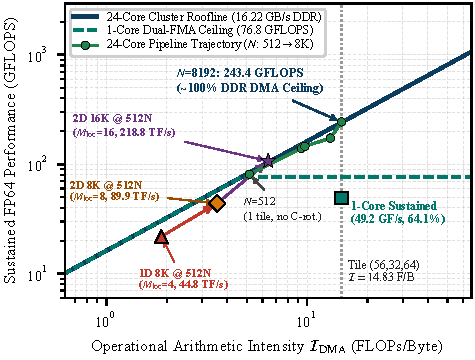
\includegraphics[width=0.75\columnwidth]{fig5_roofline_model.pdf}
    \caption{Empirical Roofline validation on an MT-3000 DSP cluster ($16.22$~GB/s DDR4 DMA ceiling, $76.8$~GFLOPS 1-core and $1{,}843.2$~GFLOPS 24-core FMA peaks), showing 1-core efficiency ($64.1\%$), 24-core saturation ($243.44$~GFLOPS), and 512-node strong-scaling operating points across 1D $8\text{K}$ ($44.8$~TF/s), 2D $8\text{K}$ ($89.9$~TF/s), and 2D $16\text{K}$ ($218.8$~TF/s).}
    \label{fig:roofline}
\end{figure}

\begin{table*}[t]
\centering
\caption{Multi-Scale Distributed Strong and Weak Scaling Across 1 to 512 MT-3000 Nodes (4 to 2,048 MPI Ranks; 96 to 49,152 DSP Cores)}
\label{tab:strong_scaling}
\renewcommand{\arraystretch}{1.06}
\setlength{\tabcolsep}{2.5pt}
\resizebox{\textwidth}{!}{%
\begin{tabular}{@{}rrrcccccccccccccc@{}}
\toprule
 & & & \multicolumn{8}{c}{\textbf{$8192^3$ Strong Scaling ($4.398$~TFLOPs): 1D Baseline vs.\ Proposed 2D Hybrid}} & \multicolumn{3}{c}{\textbf{Extreme $16384^3$ 2D Strong ($35.18$~TF)}} & \multicolumn{2}{c}{\textbf{Weak Scaling (\texttt{tri})}} \\
\cmidrule(lr){4-11} \cmidrule(lr){12-14} \cmidrule(l){15-16}
\textbf{Nodes} & \textbf{MPI} & \textbf{DSP} & \textbf{1D K.} & \textbf{1D} & \textbf{1D Comm /} & \textbf{2D K.} & \textbf{2D TF/s} & \textbf{2D \texttt{pread}} & \textbf{2D Comm /} & \textbf{2D/1D Gain} & \textbf{16K K.} & \textbf{16K TF/s} & \textbf{\texttt{pread} /} & \textbf{$2048^3$ TF/s} & \textbf{$1024^3$ / $512^3$} \\
 & \textbf{Ranks} & \textbf{Cores} & \textbf{(s)} & \textbf{TF/s} & \textbf{E2E (s)} & \textbf{(s)} & \textbf{(Eff.\ \%)} & \textbf{(s)} & \textbf{E2E (s)} & \textbf{(Kern / Comm)} & \textbf{(s)} & \textbf{(Eff.\ \%)} & \textbf{Comm (s)}$^{\S}$ & \textbf{(Eff.\ \%)}$^{\P}$ & \textbf{Eff.\ (\%)} \\
\midrule
1 & 4 & 96 & 4.5354 & 0.97 & 9.01 / 14.41 & 5.7812 & 0.76 (100\%) & 1.7782 & 2.89 / 10.45 & $0.78\times$ / $3.12\times$ & 35.7795 & 0.98 (100\%) & --- & 0.14 (100\%) & 100\% / 100\% \\
2 & 8 & 192 & 2.3148 & 1.90 & 13.94 / 16.50 & 2.8848 & 1.52 (100\%) & 1.2621 & 5.09 / 9.06 & $0.80\times$ / $2.74\times$ & 15.8621 & 2.22 (\textbf{112.8\%}) & --- & 0.28 (96.5\%) & 92.6\% / 94.2\% \\
4 & 16 & 384 & 1.2773 & 3.44 & 18.02 / 19.62 & 1.4777 & 2.98 (97.8\%) & 0.8289 & 7.10 / 9.38 & $0.86\times$ / $2.54\times$ & 9.8105 & 3.59 (91.2\%) & --- & 0.51 (89.8\%) & 88.4\% / 98.9\% \\
8 & 32 & 768 & 0.6532 & 6.73 & 18.88 / 19.58 & 0.7639 & 5.76 (94.6\%) & 0.3816 & 7.70 / 8.54 & $0.86\times$ / $2.45\times$ & 5.0231 & 7.01 (89.0\%) & 2.19 / 39.58 & 1.06 (93.2\%) & 90.8\% / 91.2\% \\
16 & 64 & 1,536 & 0.3629 & 12.12 & 20.28 / 20.73 & 0.3877 & 11.34 (\textbf{93.2\%}) & 0.1992 & 9.73 / 10.16 & $0.94\times$ / $2.08\times$ & 2.5957 & 13.56 (86.2\%) & 0.94 / 43.61 & 2.12 (93.1\%) & 83.6\% / 90.8\% \\
32 & 128 & 3,072 & 0.3319 & 13.25 & 24.26 / 24.69 & 0.2133 & 20.62 (84.7\%) & 0.1156 & 8.33 / 8.57 & $\mathbf{1.56\times}$ / $2.91\times$ & 1.3007 & 27.05 (\textbf{86.0\%}) & 0.53 / 45.29 & 4.22 (92.6\%) & 82.2\% / 88.7\% \\
64 & 256 & 6,144 & 0.1222 & 36.00 & 32.21 / 32.36 & 0.1284 & 34.26 (70.4\%) & 0.3060 & 10.26 / 10.45 & $0.95\times$ / $3.14\times$ & 0.7112 & 49.47 (78.6\%) & 0.26 / 47.40 & 8.46 (92.8\%) & 77.0\% / 54.0\% \\
128 & 512 & 12,288 & 0.1017 & 43.24 & 26.96 / 30.10 & 0.0647 & \textbf{68.01} (\textbf{69.8\%}) & \textbf{0.0406} & 8.75 / 8.85 & $\mathbf{1.57\times}$ / $3.08\times$ & 0.4223 & 83.31 (66.2\%) & 0.17 / 51.25 & 16.92 (92.8\%) & 89.5\% / \textbf{87.5\%} \\
256 & 1,024 & 24,576 & 0.0984 & 44.70 & 36.02 / 36.12 & 0.0538 & \textbf{81.77} (42.0\%) & 4.0284 & 10.43 / 10.49 & $\mathbf{1.83\times}$ / $3.45\times$ & 0.2109 & \textbf{166.82} (\textbf{66.3\%}) & \textbf{0.11} / 54.53 & 33.76 (92.6\%) & 81.6\% / 61.7\% \\
\textbf{512} & \textbf{2,048} & \textbf{49,152} & 0.0982 & 44.78 & 102.25 / 102.35 & \textbf{0.0489} & \textbf{89.92} (23.1\%) & 3.0916 & \textbf{10.32} / \textbf{10.38} & $\mathbf{2.01\times}$ / $\mathbf{9.90\times}$ & \textbf{0.1608} & \textbf{218.79} (43.5\%) & 0.12 / \textbf{47.34} & \textbf{67.24} (\textbf{92.2\%}) & \textbf{80.1\%} / 55.4\% \\
\bottomrule
\end{tabular}%
}
\vspace{1pt}
\par{\raggedright\scriptsize $^{\S}$At $1$--$4$ nodes ($M_{\mathrm{local}} \ge 2048$), $16384^3$ benchmarks use in-memory initialization because staging full $4.30$~GB unpartitioned $B$ at Rank~0 alongside $20$~GiB node DSP buffers exceeds single-node host RAM; $8$--$512$ nodes execute full storage-to-DSP \texttt{pread} + subgroup collectives. $^{\P}$At 512 nodes ($2048^3$ weak scaling), tri-buffering (\texttt{pipeline\_opt}) reaches $92.21\%$ ($0.5233$~s, $67.24$~TF/s) vs.\ double buffering's $89.64\%$ ($0.5382$~s, $65.38$~TF/s, $+2.77\%$ gain).\par}
\end{table*}

\begin{figure*}[t]
    \centering
    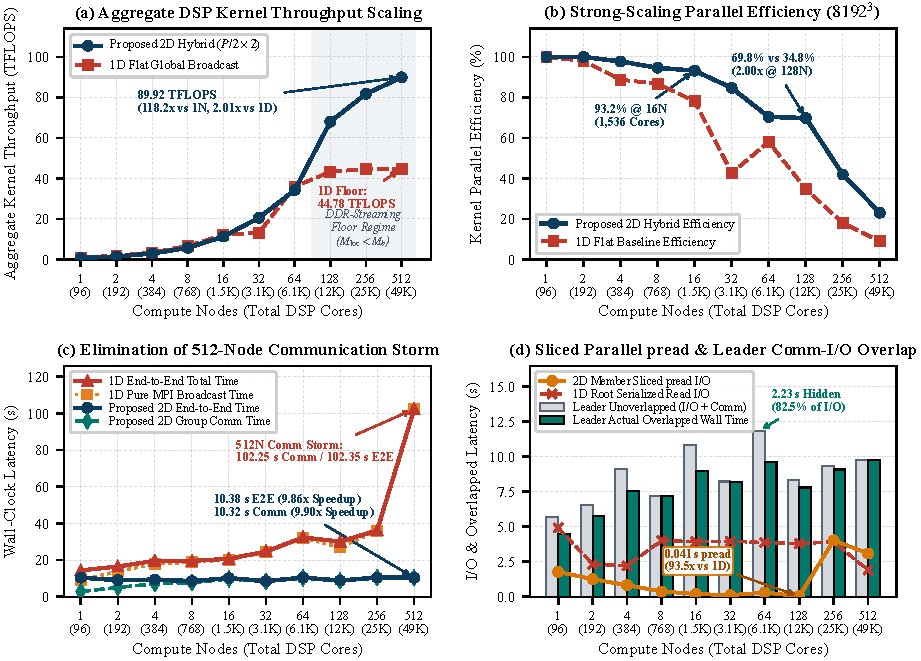
\includegraphics[width=0.44\textwidth]{fig6_strong_scaling_512nodes.pdf}
    \caption{Strong-scaling evaluation of $8192^3$ complex GEMM across 1 to 512 MT-3000 supercomputer nodes (4 to 2,048 MPI ranks; 96 to 49,152 DSP cores): (a) aggregate DSP kernel throughput showing the 1D DDR-streaming floor ($44.78$~TFLOPS) vs.\ our 2D hybrid breakthrough ($89.92$~TFLOPS, $2.01\times$); (b) kernel strong-scaling parallel efficiency; (c) elimination of the 512-node $102.25$~s MPI broadcast storm ($9.90\times$ comm speedup, $9.86\times$ E2E speedup); (d) member sliced parallel \texttt{pread} latency ($93.5\times$ speedup at 128 nodes) and leader communication-I/O overlap ($82.5\%$ I/O hidden at 64 nodes).}
    \label{fig:strong_scaling}
\end{figure*}

\begin{figure*}[t]
    \centering
    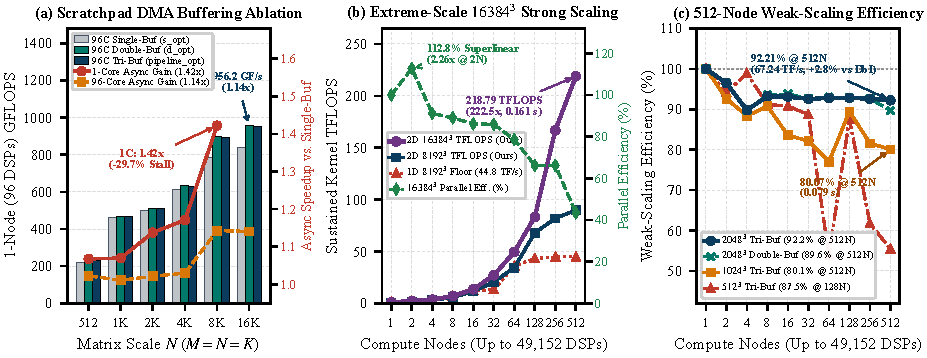
\includegraphics[width=0.63\textwidth]{fig7_ablation_extreme_weak.pdf}
    \caption{Micro-architectural ablation and extreme-scale evaluation up to 512 nodes (49,152 DSP cores): (a) single/double/tri-buffered scratchpad DMA ablation reaching $956.17$~GFLOPS/node and $1.42\times$ 1-core async speedup; (b) extreme-scale $16384^3$ ($35.184$~TFLOPs) vs.\ $8192^3$ strong scaling achieving $218.79$~TFLOPS ($222.49\times$ speedup) and $112.80\%$ 2-node superlinear efficiency; (c) 1--512 node weak-scaling efficiency sustaining $92.21\%$ ($67.24$~TFLOPS, $+2.77\%$ over double buffering) at 49,152 DSP cores.}
    \label{fig:ablation_extreme_weak}
\end{figure*}

\subsection{Experimental Setup and Methodology}
We evaluate our framework on an MT-3000 supercomputer scaling from $1$ to $512$ compute nodes, harnessing up to \textbf{8,192 ARMv8 GP cores, 2,048 MPI processes, 2,048 autonomous DSP clusters, 49,152 bare-metal DSP cores, and 786,432 FP64 VPU SIMD lanes} ($5.94$~PFLOPS aggregate chip-level peak). Host code is compiled with \texttt{mpicc -O2 -fopenmp} linked against Hthread and OpenBLAS; DSP kernels use the vendor VLIW/SIMD C compiler with explicit \texttt{lvector} and \texttt{dma\_p2p} intrinsics.

All benchmarks execute IEEE-754 FP64 complex arithmetic ($8MNK$ FLOPs) across four campaigns: (1) \emph{intra-node comparisons} ($N \in [512, 16384]$) against ARMv8 OpenBLAS~\cite{zhang2012openblas} under planar \textbf{\texttt{4x DGEMM}} and interleaved AoS \textbf{\texttt{1x ZGEMM}}; (2) \emph{scratchpad DMA buffering ablation} (\texttt{gemm\_host\_ASR}) isolating single-buffered (\texttt{s\_opt}), $A/B$ double-buffered (\texttt{d\_opt}), and 14-channel tri-buffered (\texttt{pipeline\_opt}) kernels sharing the identical $4 \times 4$ 32-VR micro-kernel across 1 core, 1 cluster (24C), and 1 node (96C, 4 ranks); (3) \emph{multi-scale strong scaling} ($1$--$512$ nodes) at $8192^3$ ($4.398$~TFLOPs) and extreme $16384^3$ ($35.184$~TFLOPs); and (4) \emph{1--512 node weak scaling} under constant per-node base workloads ($512^3 = 1.07$~GFLOPs, $1024^3 = 8.59$~GFLOPs, and $2048^3 = 68.72$~GFLOPs/node, reaching $35.184$~TFLOPs at 512 nodes). Distributed times record maximum wall-clock latency across ranks via \texttt{MPI\_Barrier} and \texttt{MPI\_Wtime}.

\subsection{Intra-Node Throughput and Accuracy vs.\ OpenBLAS}
Table~\ref{tab:intra_node} and Fig.~\ref{fig:intra_node} report intra-node throughput and precision:

\textbf{1) Single-Core Compute Density:} One MT-3000 DSP core running our tri-buffered $4 \times 4$ micro-kernel sustains \textbf{$44.16$--$49.19$~GFLOPS} across all scales, reaching \textbf{$64.1\%$ of its $76.8$~GFLOPS dual-FMA peak}. Because 1 core's bandwidth demand ($49.19 / 14.83 = 3.32$~GB/s) lies well below the cluster's $16.22$~GB/s DDR4 DMA ceiling, 1-core execution is compute-bound, outperforming 1-core ARMv8 OpenBLAS by \textbf{$6.12\times$--$7.28\times$} (\texttt{4x DGEMM}) and \textbf{$5.95\times$--$6.47\times$} (\texttt{1x ZGEMM}).

\textbf{2) Single-Cluster vs.\ Multi-Core CPU Scaling:} Pairing 16 ARMv8 cores with 4 DSP clusters makes \emph{4 ARMv8 cores} the exact cluster-equivalent host resource ($1/4$ node GP vs.\ $1/4$ node ACC). One 24-core DSP cluster reaches \textbf{$243.44$~GFLOPS} at $N=8192$ ($18.066$~s), achieving a \textbf{$9.33\times$ speedup} over 4-core OpenBLAS ($26.08$~GFLOPS). Even against \emph{all 16 ARMv8 cores}, one DSP cluster ($25\%$ of ACC) beats 16-core \texttt{1x ZGEMM} ($89.65$~GFLOPS) by \textbf{$2.72\times$} ($10.86\times$ node-equivalent) and 16-core \texttt{4x DGEMM} ($44.56$~GFLOPS) by \textbf{$5.46\times$} at $N=8192$ and \textbf{$6.57\times$} at $N=16384$ ($199.21$ vs.\ $30.34$~GFLOPS, where 16-core \texttt{4x DGEMM} thrashes LLC/NUMA and \texttt{1x ZGEMM} hits OOM from $12$~GiB AoS buffers, while our $2 \times 2$ host-tiled planar schedule runs workspace-free).

\textbf{3) IEEE-754 FP64 Numerical Accuracy:} Across all $6.71 \times 10^7$ complex outputs at $N=8192$ (and Tile~0 at $N=16384$), maximum $\ell_\infty$ error against OpenBLAS scales as $\mathcal{O}(K \epsilon_{\mathrm{FP64}})$ (Fig.~\ref{fig:intra_node}(c)), bounded within $7.28 \times 10^{-12}$--$2.18 \times 10^{-8}$ (well below FP32 $\epsilon_{\mathrm{mach}} = 1.19 \times 10^{-7}$), confirming exact fused FMA accumulation without 3M cancellation.

\subsection{Scratchpad DMA Buffering Ablation and Roofline Validation}
Table~\ref{tab:dma_ablation}, Fig.~\ref{fig:roofline}, and Fig.~\ref{fig:ablation_extreme_weak}(a) isolate asynchronous DMA pipelining gains and validate our Roofline model:

\textbf{1) Single vs.\ Double vs.\ Tri-Buffering Ablation:} With the $4 \times 4$ 32-VR micro-kernel fixed, single-buffered \texttt{s\_opt} serializes DDR4$\leftrightarrow$SM/AM DMA with VPU compute. On 1 DSP core, as $N$ reaches $8192$ and outer DDR4 stride penalties grow, \texttt{s\_opt} drops from $43.23$ to $33.79$~GFLOPS ($130.17$~s), whereas asynchronous ping-pong overlap (\texttt{d\_opt}) sustains \textbf{$48.05$~GFLOPS} ($91.52$~s)---a \textbf{$1.422\times$ speedup ($29.69\%$ wall-time cut)}. Across 1 cluster (24C) and 1 full node (96C, 4 MPI ranks in a $2 \times 2$ grid), asynchronous DMA buffering yields a steady \textbf{$1.141\times$--$1.144\times$ speedup} ($12.4\%$--$12.6\%$ time savings) at $N \ge 8192$, raising 96-core single-node throughput from $783.47$ to \textbf{$895.84$~GFLOPS} at $N=8192$ and from $838.03$ to \textbf{$956.17$~GFLOPS} at $N=16384$ ($36.80$~s vs.\ $41.98$~s). On a quiet single node, \texttt{d\_opt} and \texttt{pipeline\_opt} agree within $<\!0.9\%$ ($956.17$ vs.\ $953.54$~GFLOPS) due to minor 14-channel modulo descriptor overhead, whereas at 512-node scale (Section~\ref{sec:eval_weak}), \texttt{pipeline\_opt}'s cyclic $C$-tile triple buffer provides decisive jitter resilience.

\textbf{2) Empirical Roofline Saturation:} In Fig.~\ref{fig:roofline}, as $N$ grows from $512$ ($1$ partial tile/core, no $C$-rotation, $80.98$~GFLOPS) to $8192$ ($5$--$6$ full 64-column tiles/core at $\mathcal{I}_{\mathrm{DMA}} = 14.83$~FLOPs/Byte), 24-core throughput climbs along the $16.22$~GB/s DDR4 slope to \textbf{$243.44$~GFLOPS}, matching our $240.5$~GFLOPS ceiling in~\eqref{eq:cluster_roofline} within $1.2\%$ ($\sim\!100\%$ DDR4 DMA saturation). Across 4 clusters per node, the theoretical node ceiling $4 \times 240.5 = \mathbf{962.0~\text{GFLOPS}}$ matches our measured 96-core throughput of \textbf{$956.17$~GFLOPS} within $0.6\%$, while all three 512-node operating points---1D $8\text{K}$ ($\mathcal{I}\!=\!1.88, 44.78$~TF/s), 2D $8\text{K}$ ($\mathcal{I}\!=\!3.56, 89.92$~TF/s), and 2D $16\text{K}$ ($\mathcal{I}\!=\!6.40, 218.79$~TF/s)---align closely along the 2,048-cluster DMA Roofline.

\subsection{Multi-Scale Strong Scaling: $8192^3$ and Extreme $16384^3$}
\label{sec:eval_scaling}
Table~\ref{tab:strong_scaling}, Fig.~\ref{fig:strong_scaling}, and Fig.~\ref{fig:ablation_extreme_weak}(b) evaluate strong scaling across 1 to 512 nodes (96 to 49,152 DSP cores):

\textbf{1) $8192^3$ DDR-Floor Breakthrough and $9.90\times$ Collective Storm Elimination:} At $1$--$16$ nodes ($M_{\mathrm{local}} \ge 128 > M_b$), our 2D scheme sustains \textbf{$93.19\%$ parallel efficiency} ($0.76 \to 11.34$~TFLOPS) and runs $1.38\times$--$2.29\times$ faster end-to-end than 1D. Beyond $64$ nodes, 1D crosses $M_{\mathrm{local}} < 32$ and stalls at the DDR4 streaming floor~\eqref{eq:ddr_floor} (\textbf{$0.0982$~s, $44.78$~TFLOPS, $9.02\%$ efficiency} at 512 nodes), while its global broadcast detonates into a \textbf{$102.25$~s storm} ($102.35$~s E2E). Doubling $M_{\mathrm{local}}$ ($4 \to 8$) and halving $B_g$ traffic enables our 2D co-design to sustain \textbf{$69.84\%$ efficiency at 128 nodes ($68.01$~TFLOPS)} and reach \textbf{$0.0489$~s ($89.92$~TFLOPS, $118.20\times$ over 1 node)} at 512 nodes---an exact \textbf{$2.01\times$ kernel speedup} validating~\eqref{eq:ddr_floor}---while subgroup \texttt{MPI\_Ibcast} holds 512-node communication flat at \textbf{$10.32$~s ($9.90\times$ comm; $10.38$~s E2E, $9.86\times$ speedup)}. Sliced parallel \texttt{pread} cuts member I/O to \textbf{$0.0406$~s at 128 nodes ($93.5\times$ over 1D)} and hides \textbf{$2.23$~s ($82.5\%$)} of leader I/O behind Phase-1 transfers at 64 nodes (Fig.~\ref{fig:strong_scaling}(d)).

\textbf{2) Extreme-Scale $16384^3$ Strong Scaling to $218.79$~TFLOPS:} Scaling $M\!=\!N\!=\!K\!=\!16384$ ($35.184$~TFLOPs) across 1 to 512 nodes demonstrates two key phenomena (Table~\ref{tab:strong_scaling}, Fig.~\ref{fig:ablation_extreme_weak}(b)). First, scaling from 1 node ($35.7795$~s, $0.983$~TFLOPS, $M_{\mathrm{local}}\!=\!8192$) to 2 nodes ($15.8621$~s, $2.218$~TFLOPS, $M_{\mathrm{local}}\!=\!4096$) yields a \textbf{superlinear $2.256\times$ speedup ($112.80\%$ efficiency)} as halving per-cluster $A_r/C_{r,g}$ footprint ($4.0 \to 2.0$~GiB) relieves 4-cluster shared DDR4 bank/page contention. Second, efficiency holds above \textbf{$85.96\%$ through 32 nodes} ($27.05$~TFLOPS, $27.51\times$) and \textbf{$66.26\%$ through 256 nodes} ($0.2109$~s, \textbf{$166.82$~TFLOPS}, $169.64\times$). At 512 nodes (49,152 DSPs, $M_{\mathrm{local}}\!=\!16$), kernel runtime compresses to \textbf{$0.1608$~s}, reaching \textbf{$218.79$~TFLOPS} (\textbf{$222.49\times$ speedup}, $43.45\%$ efficiency, $2.43\times$ over $8192^3$). Across 8--512 nodes, subgroup broadcast of the $4.30$~GB complex $B$ matrix stays storm-free ($39.58$--$47.34$~s), while parallel \texttt{pread} reduces member I/O from $2.1881$~s (8N) to \textbf{$0.1117$~s} (256N) and \textbf{$0.1235$~s} (512N, $37.9\times$ faster than leader I/O).

\subsection{512-Node Weak Scaling and Tri-Buffer Jitter Resilience}
\label{sec:eval_weak}
Table~\ref{tab:strong_scaling} and Fig.~\ref{fig:ablation_extreme_weak}(c) evaluate 1--512 node weak scaling:
\begin{itemize}\setlength{\itemsep}{0.5pt}\setlength{\parskip}{0pt}
    \item \textbf{$2048^3$ Base Workload ($68.72$~GFLOPs/node $\to 35.184$~TFLOPs @ 512N):} Runtime stays nearly flat across a $512\times$ scale-out, rising by just $40.7$~ms from $0.4825$~s (1N) to \textbf{$0.5233$~s at 512N} ($67.24$~TFLOPS) to sustain \textbf{$92.21\%$--$93.21\%$ efficiency} across 8--512 nodes (\textbf{$92.21\%$ at 49,152 DSPs}). While \texttt{d\_opt} and \texttt{pipeline\_opt} tie at 1 node ($0.4824$~s vs.\ $0.4825$~s), at 512 nodes \texttt{d\_opt} slips to $0.5382$~s ($89.64\%$, $65.38$~TFLOPS), proving that cyclic $C$-tile triple buffering yields \textbf{$+2.77\%$ higher throughput ($+2.57$ percentage points)} by absorbing DDR/NIC jitter.
    \item \textbf{$1024^3$ and Ultra-Fine $512^3$ Workloads:} For sub-$80$~ms $1024^3$ tasks ($8.59$~GFLOPs/node), \texttt{pipeline\_opt} sustains \textbf{$80.07\%$ efficiency at 512 nodes} ($0.0631 \to 0.0788$~s vs.\ \texttt{d\_opt}'s $78.50\%$). Even for $13.8$~ms $512^3$ tasks ($1.07$~GFLOPs/node), \texttt{pipeline\_opt} holds \textbf{$87.51\%$ efficiency at 128 nodes} ($12{,}288$ DSPs; $55.39\%$ vs.\ $52.22\%$ at 512N).
\end{itemize}

% ============================================================================
\section{Related Work}
\label{sec:related}
% ============================================================================
\textbf{Dense and Complex BLAS Micro-Kernels:} CPU GEMM libraries---ATLAS~\cite{whaley2001atlas}, GotoBLAS~\cite{goto2008anatomy}, OpenBLAS~\cite{zhang2012openblas}, and BLIS~\cite{vanzee2015blis}---rely on hierarchical cache-blocking and register-resident micro-kernels tailored to hardware caches, including 3M/4M complex GEMM in BLIS~\cite{vanzee2017complex}. Unlike cache-coherent CPUs, MT-3000 DSP cores expose bare-metal $64$~KB SM and $768$~KB AM scratchpads without hardware cache refill, requiring explicit 14-channel DMA triple/double buffering alongside split-complex hoisted-negation \texttt{vec\_svbcast} FMA scheduling.

\textbf{Scratchpad Many-Core and MT-3000 Optimizations:} Software-managed DMA double buffering was pioneered on IBM Cell BE~\cite{kahle2005cell}, TI C6678 DSPs~\cite{igual2012dsp}, and Sunway SW26010~\cite{fu2016sunway, jiang2017sw26010}. On MT-3000, Lu~\emph{et~al.}~\cite{lu2022mt3000} introduced the multi-zone architecture, Li~\emph{et~al.}~\cite{li2024md} ported molecular dynamics kernels, Fang~\emph{et~al.}~\cite{fang2026mtgemm} developed \texttt{mtGEMM} for single-cluster real DGEMM, Mo~\emph{et~al.}~\cite{mo2024irregular} studied irregular single-cluster GEMM, and Qi~\emph{et~al.}~\cite{qi2025constraint, qi2026attention} explored single-cluster auto-tuning for real GEMM-like and attention operators. None address FP64 \emph{complex} GEMM, $C$-matrix cyclic triple buffering, or \emph{multi-node strong/weak scaling} across tens of thousands of DSPs.

\textbf{Distributed GEMM and Collective Algorithms:} ScaLAPACK~\cite{choi1996scalapack}, SUMMA~\cite{vandegeijn1997summa}, 2.5D GEMM~\cite{solomonik2011comm25d}, COSMA~\cite{kwasniewski2019cosma}, and SLATE~\cite{gates2019slate} optimize communication on homogeneous CPU/GPU grids, while MPICH~\cite{thakur2005mpich} and hierarchical collectives~\cite{parsons2014hierarchical} optimize tree topologies. Our Stationary-$A$, Panel-Broadcast-$B$ 2D co-design uniquely couples zero-copy strided \texttt{MPI\_Type\_vector} subgroup collectives with parallel POSIX \texttt{pread} into DSP-pinned memory and 64-column SIMD alignment to suppress 2,048-rank storms and halve the DDR floor.

% ============================================================================
\section{Discussion and Conclusion}
\label{sec:conclusion}
% ============================================================================
\textbf{Portability Beyond $N=16384$:} Our co-design generalizes directly to broader multi-zone scratchpad accelerators (e.g., Sunway SW26010-Pro, multi-cluster DSPs, and spatial dataflow tiles). The constraint $N/G \ge 24 \times 3 N_b = 4{,}608$ ($Q \ge 64$) governs optimal panel count $G$: while $G=2$ is optimal at $N=8192$ and reaches $218.79$~TFLOPS at $N=16384$, $N \ge 32768$ permits $G \in \{8, 16\}$, cutting subgroup broadcast payloads and the DDR floor~\eqref{eq:ddr_floor} by $8\times$--$16\times$, while node-level shared-memory I/O leaders can curb Lustre contention above $1{,}024$ readers.

\textbf{Conclusion:} We presented an end-to-end hierarchical co-design for distributed FP64 complex GEMM on MT-3000 supercomputers. Uniting a 14-channel asynchronous DMA tri-buffered scratchpad pipeline and a $4 \times 4$ 32-VR dual-FMA micro-kernel ($86.1\%$ AM vector traffic cut) with Stationary-$A$, Panel-Broadcast-$B$ 2D collectives and parallel \texttt{pread} achieves $49.19$~GFLOPS/core ($1.42\times$ async DMA speedup; $6.12\times$--$7.28\times$ over 1-core OpenBLAS), saturates $\sim\!100\%$ of the $240.5$~GFLOPS cluster DDR4 Roofline ($243.44$~GFLOPS/cluster, $956.17$~GFLOPS/node), cuts 512-node collective time by $9.90\times$ ($102.25 \to 10.32$~s), reaches $89.92$~TFLOPS ($8192^3$) and $218.79$~TFLOPS ($16384^3$, $222.49\times$ speedup), and sustains $92.21\%$ weak-scaling efficiency across 512 nodes (49,152 DSPs).

\clearpage
\IEEEtriggeratref{14}
\bibliographystyle{IEEEtran}
\bibliography{references}

\end{document}
